\section{ระบบขับเคลื่อนหุ่นยนต์และเซอร์โวแอมปลิไฟเออร์}

\textbf{ชื่อบทภาษาอังกฤษ:} Robot Drive Systems and Servo Amplifiers \\
\textbf{รายวิชา:} หุ่นยนต์ในระบบงานอุตสาหกรรม (Industrial Robots) \\
\textbf{รหัสวิชา:} 5574506 \\
\textbf{หน่วยกิต:} 3(1-4-4) \\
\textbf{ระดับผู้เรียน:} นักศึกษาระดับปริญญาตรี \\
\textbf{จำนวนชั่วโมงที่แนะนำ:} บรรยาย 2 ชั่วโมง ปฏิบัติ 8 ชั่วโมง และศึกษาด้วยตนเอง 8 ชั่วโมง \\

\begin{quote}
    \textbf{ขอบเขตของบท:} ระบบขับเคลื่อนด้วยไฟฟ้า นิวเมติก และไฮดรอลิก มอเตอร์กระแสตรง มอเตอร์สเต็ปเปอร์ มอเตอร์เซอร์โว Encoder, Resolver, Servo Drive และ Servo Amplifier ตลอดจนการควบคุมแรงบิด ความเร็ว และตำแหน่งของแกนหุ่นยนต์อุตสาหกรรม
\end{quote}

\par\noindent\rule{\textwidth}{0.4pt}\par

\subsection{แนวคิดสำคัญของบท}

ระบบขับเคลื่อนหุ่นยนต์ (Robot Drive System) เป็นส่วนที่เปลี่ยนพลังงานให้เป็นการเคลื่อนที่ของข้อต่อและแกนต่าง ๆ ของหุ่นยนต์อุตสาหกรรม คุณภาพของระบบขับเคลื่อนมีผลโดยตรงต่อความแม่นยำ ความเร็ว ความราบรื่น กำลังรับโหลด ความสามารถในการทำซ้ำตำแหน่ง และความปลอดภัยของระบบ หุ่นยนต์สมัยใหม่จึงไม่ได้พิจารณาเฉพาะชนิดของมอเตอร์ แต่ต้องพิจารณาร่วมกันทั้งแหล่งพลังงาน มอเตอร์หรือกระบอกสูบ ชุดส่งกำลัง ตัวตรวจจับป้อนกลับ อุปกรณ์ขยายกำลัง และอัลกอริทึมควบคุม

ระบบขับเคลื่อนหลักแบ่งได้เป็นสามกลุ่ม ได้แก่ ระบบไฟฟ้า ระบบนิวเมติก และระบบไฮดรอลิก ระบบไฟฟ้าได้รับความนิยมสูงในหุ่นยนต์อุตสาหกรรมทั่วไปเนื่องจากควบคุมตำแหน่งและความเร็วได้ละเอียด เชื่อมต่อกับตัวควบคุมดิจิทัลได้สะดวก และดูแลรักษาง่าย ระบบนิวเมติกเหมาะกับการเคลื่อนที่แบบสองตำแหน่ง งานหยิบจับ และอุปกรณ์ปลายแขนที่ต้องการความเรียบง่าย ส่วนระบบไฮดรอลิกเหมาะกับงานที่ต้องการแรงหรือแรงบิดสูงมาก แต่ต้องจัดการปั๊ม วาล์ว ของไหล การรั่วซึม และการบำรุงรักษาอย่างเหมาะสม

หัวใจของระบบเซอร์โวคือการควบคุมแบบวงปิด (Closed-Loop Control) ตัวควบคุมส่งคำสั่งไปยัง Servo Drive หรือ Servo Amplifier อุปกรณ์ดังกล่าวแปลงพลังงานไฟฟ้าและควบคุมกระแสที่จ่ายให้มอเตอร์ ขณะเดียวกัน Encoder หรือ Resolver จะวัดตำแหน่งและความเร็วจริงส่งกลับมาเปรียบเทียบกับค่าคำสั่ง ความคลาดเคลื่อนที่เกิดขึ้นถูกใช้ในการปรับแรงบิด ความเร็ว และตำแหน่งอย่างต่อเนื่อง

ระบบเซอร์โวอุตสาหกรรมโดยทั่วไปประกอบด้วยวงรอบควบคุมซ้อนกัน ได้แก่ วงรอบกระแสหรือแรงบิดเป็นวงรอบชั้นใน วงรอบความเร็วเป็นชั้นกลาง และวงรอบตำแหน่งเป็นชั้นนอก วงรอบชั้นในต้องตอบสนองเร็วกว่าวงรอบชั้นนอกเพื่อให้ระบบมีเสถียรภาพและตอบสนองต่อการรบกวนได้ดี เอกสารทางเทคนิคของ Texas Instruments อธิบายว่าวงรอบกระแสเป็นฐานของสมรรถนะวงรอบความเร็วและตำแหน่ง และในระบบจำนวนมากแบนด์วิดท์ของวงรอบกระแสจะสูงกว่าวงรอบชั้นนอกอย่างมีนัยสำคัญ [3]

\par\noindent\rule{\textwidth}{0.4pt}\par

\subsection{ความรู้พื้นฐานก่อนเรียน}

ก่อนเรียนบทนี้ นักศึกษาควรมีความรู้หรือทักษะดังต่อไปนี้

\begin{enumerate}
    \item หลักการพื้นฐานของหุ่นยนต์อุตสาหกรรม ข้อต่อ แกน และพิกัดการเคลื่อนที่
    \item กฎของโอห์ม กำลังไฟฟ้า และวงจรไฟฟ้ากระแสตรงเบื้องต้น
    \item แนวคิดของแรง แรงบิด ความเร็วเชิงมุม ความเร่ง และโมเมนต์ความเฉื่อย
    \item หลักการควบคุมแบบวงเปิดและวงปิด
    \item การอ่านแผนภาพบล็อก แผนผังวงจร และข้อมูลพิกัดจากคู่มือผู้ผลิต
    \item ความปลอดภัยพื้นฐานในห้องปฏิบัติการไฟฟ้า เครื่องกล และระบบอัตโนมัติ
\end{enumerate}

\par\noindent\rule{\textwidth}{0.4pt}\par

\subsection{คำสำคัญประจำบท}

\begin{table}[htbp]
    \centering
    \begin{tabular}{l l l}
        \hline
        \textbf{คำศัพท์ภาษาไทย} & \textbf{คำศัพท์ภาษาอังกฤษ} & \textbf{ความหมายโดยย่อ} \\
        \hline
        ระบบขับเคลื่อนหุ่นยนต์ & Robot Drive System & ระบบที่สร้างและส่งแรงหรือแรงบิดไปยังแกนของหุ่นยนต์ \\
        ตัวกระทำ & Actuator & อุปกรณ์ที่เปลี่ยนพลังงานเป็นการเคลื่อนที่ \\
        เซอร์โวมอเตอร์ & Servo Motor & มอเตอร์ที่ทำงานร่วมกับตัวตรวจจับและวงรอบควบคุม \\
        เซอร์โวไดรฟ์ & Servo Drive & อุปกรณ์อิเล็กทรอนิกส์กำลังและตัวควบคุมสำหรับขับมอเตอร์เซอร์โว \\
        เซอร์โวแอมปลิไฟเออร์ & Servo Amplifier & ส่วนขยายกำลังของระบบเซอร์โว; ในงานอุตสาหกรรมมักใช้เรียกแทน Servo Drive \\
        เอ็นโค้ดเดอร์ & Encoder & ตัวตรวจจับที่แปลงการเคลื่อนที่เป็นสัญญาณตำแหน่งหรือความเร็ว \\
        รีโซลเวอร์ & Resolver & ตัวตรวจจับตำแหน่งเชิงมุมแบบแม่เหล็กไฟฟ้าที่ให้สัญญาณไซน์และโคไซน์ \\
        แรงบิด & Torque & ผลของแรงที่ทำให้วัตถุหมุน มีหน่วยนิวตัน–เมตร \\
        โมเมนต์ความเฉื่อย & Moment of Inertia & สมบัติที่ต้านการเปลี่ยนแปลงความเร็วเชิงมุม \\
        วงรอบกระแส & Current Loop & วงรอบชั้นในที่ควบคุมกระแสและแรงบิด \\
        วงรอบความเร็ว & Velocity Loop & วงรอบที่ควบคุมความเร็วเพลา \\
        วงรอบตำแหน่ง & Position Loop & วงรอบชั้นนอกที่ควบคุมตำแหน่งแกน \\
        อัตราทด & Gear Ratio & อัตราส่วนความเร็วด้านมอเตอร์ต่อความเร็วด้านโหลด \\
        แรงบิดพิกัดต่อเนื่อง & Continuous Torque & แรงบิดที่จ่ายได้ต่อเนื่องโดยไม่เกินขีดจำกัดความร้อน \\
        แรงบิดสูงสุดชั่วขณะ & Peak Torque & แรงบิดสูงที่อนุญาตในช่วงเวลาสั้น \\
        การปรับจูน & Servo Tuning & การตั้งค่าพารามิเตอร์ควบคุมให้ตอบสนองเร็ว เสถียร และไม่สั่น \\
        ความละเอียด & Resolution & การเปลี่ยนแปลงตำแหน่งที่เล็กที่สุดซึ่งตัวตรวจจับแยกได้ \\
        ความถูกต้อง & Accuracy & ความใกล้เคียงระหว่างค่าที่วัดกับค่าจริง \\
        ความสามารถทำซ้ำ & Repeatability & ความสามารถกลับมายังตำแหน่งเดิมซ้ำ ๆ \\
        Safe Torque Off & STO & ฟังก์ชันที่ป้องกันการสร้างแรงบิดของมอเตอร์ \\
        \hline
    \end{tabular}
\end{table}

\par\noindent\rule{\textwidth}{0.4pt}\par

\subsection{ผลลัพธ์การเรียนรู้ประจำบท}

เมื่อเรียนจบบทนี้ นักศึกษาสามารถ

\begin{enumerate}
    \item \textbf{อธิบาย} โครงสร้าง หน้าที่ และความสัมพันธ์ขององค์ประกอบในระบบขับเคลื่อนหุ่นยนต์ได้
    \item \textbf{จำแนกและเปรียบเทียบ} ระบบขับเคลื่อนด้วยไฟฟ้า นิวเมติก และไฮดรอลิกตามกำลัง ความแม่นยำ ความเร็ว การบำรุงรักษา และความเหมาะสมของงานได้
    \item \textbf{คำนวณ} แรง แรงบิด ความเร็ว อัตราทด ความละเอียด และพารามิเตอร์พื้นฐานของมอเตอร์ กระบอกสูบ และตัวตรวจจับได้
    \item \textbf{วิเคราะห์} การทำงานของ Encoder, Resolver, Servo Drive และวงรอบควบคุมแรงบิด ความเร็ว และตำแหน่งได้
    \item \textbf{เลือก} ชนิดตัวขับ มอเตอร์ ตัวตรวจจับ และอัตราทดเบื้องต้นให้เหมาะกับภาระงานของแกนหุ่นยนต์ได้
    \item \textbf{ทดลองและประเมิน} การตอบสนองของระบบขับเคลื่อนหรือชุดฝึกเซอร์โวอย่างปลอดภัย พร้อมบันทึกและอภิปรายผลได้
\end{enumerate}

\par\noindent\rule{\textwidth}{0.4pt}\par

\subsection{แผนผังเนื้อหาของบท}

ระบบขับเคลื่อนหุ่นยนต์ \\
\texttt{>} การจำแนกตามแหล่งพลังงาน \\
\texttt{>} ระบบไฟฟ้า นิวเมติก และไฮดรอลิก \\
\texttt{>} มอเตอร์ DC, Stepper และ Servo \\
\texttt{>} Encoder และ Resolver \\
\texttt{>} Servo Drive / Servo Amplifier \\
\texttt{>} วงรอบแรงบิด ความเร็ว และตำแหน่ง \\
\texttt{>} ชุดเกียร์ อัตราทด และโมเมนต์ความเฉื่อยสะท้อน \\
\texttt{>} การเลือกขนาด การตั้งค่า และการปรับจูน \\
\texttt{>} การทดลอง การประเมินสมรรถนะ และความปลอดภัย

% [รูปที่ 1: ภาพรวมระบบขับเคลื่อนหุ่นยนต์อุตสาหกรรม]
% ประเภทภาพ: Infographic / Block Diagram
% ตำแหน่งที่แนะนำ: หลังหัวข้อ 5
% วัตถุประสงค์การเรียนรู้: แสดงความสัมพันธ์ตั้งแต่คำสั่งการเคลื่อนที่ไปจนถึงการเคลื่อนที่ของข้อต่อและสัญญาณป้อนกลับ
% คำอธิบายภาพ: Robot Controller ส่งคำสั่งตำแหน่ง ความเร็ว หรือแรงบิดไปยัง Servo Drive จากนั้นจ่ายกำลังไปยัง Servo Motor ผ่านชุดเกียร์ไปยัง Robot Joint และมี Encoder/Resolver ส่งสัญญาณป้อนกลับ พร้อมกรอบเปรียบเทียบ Pneumatic Cylinder และ Hydraulic Actuator
% องค์ประกอบที่ต้องมี: Robot Controller, Servo Drive/Amplifier, Motor, Gearbox, Joint, Encoder/Resolver, Power Source, Feedback Arrow, Pneumatic, Hydraulic
% ข้อความหรือป้ายกำกับ: Position Command, Speed Command, Torque Command, Power Conversion, Mechanical Motion, Feedback
% ภาษาของป้ายกำกับ: ไทยและอังกฤษ
% สัดส่วนภาพ: 16:9
% Image Generation Prompt: Clean academic engineering infographic showing an industrial robot drive architecture. Robot controller sends position, speed, and torque commands to a servo drive/amplifier, which converts electrical power and drives a servo motor. The motor connects through a gearbox to a robot joint. An encoder or resolver returns position and speed feedback to the drive. Add small side panels comparing pneumatic cylinder and hydraulic actuator alternatives. Clear arrows, technically correct labels, blue-white industrial textbook style, bilingual Thai-English labels, no decorative clutter, 16:9.
% Alt Text: แผนภาพระบบควบคุมแกนหุ่นยนต์จากตัวควบคุมผ่านเซอร์โวไดรฟ์ มอเตอร์ ชุดเกียร์ และข้อต่อ พร้อมเส้นป้อนกลับ

\begin{figure}[htbp]
    \centering
    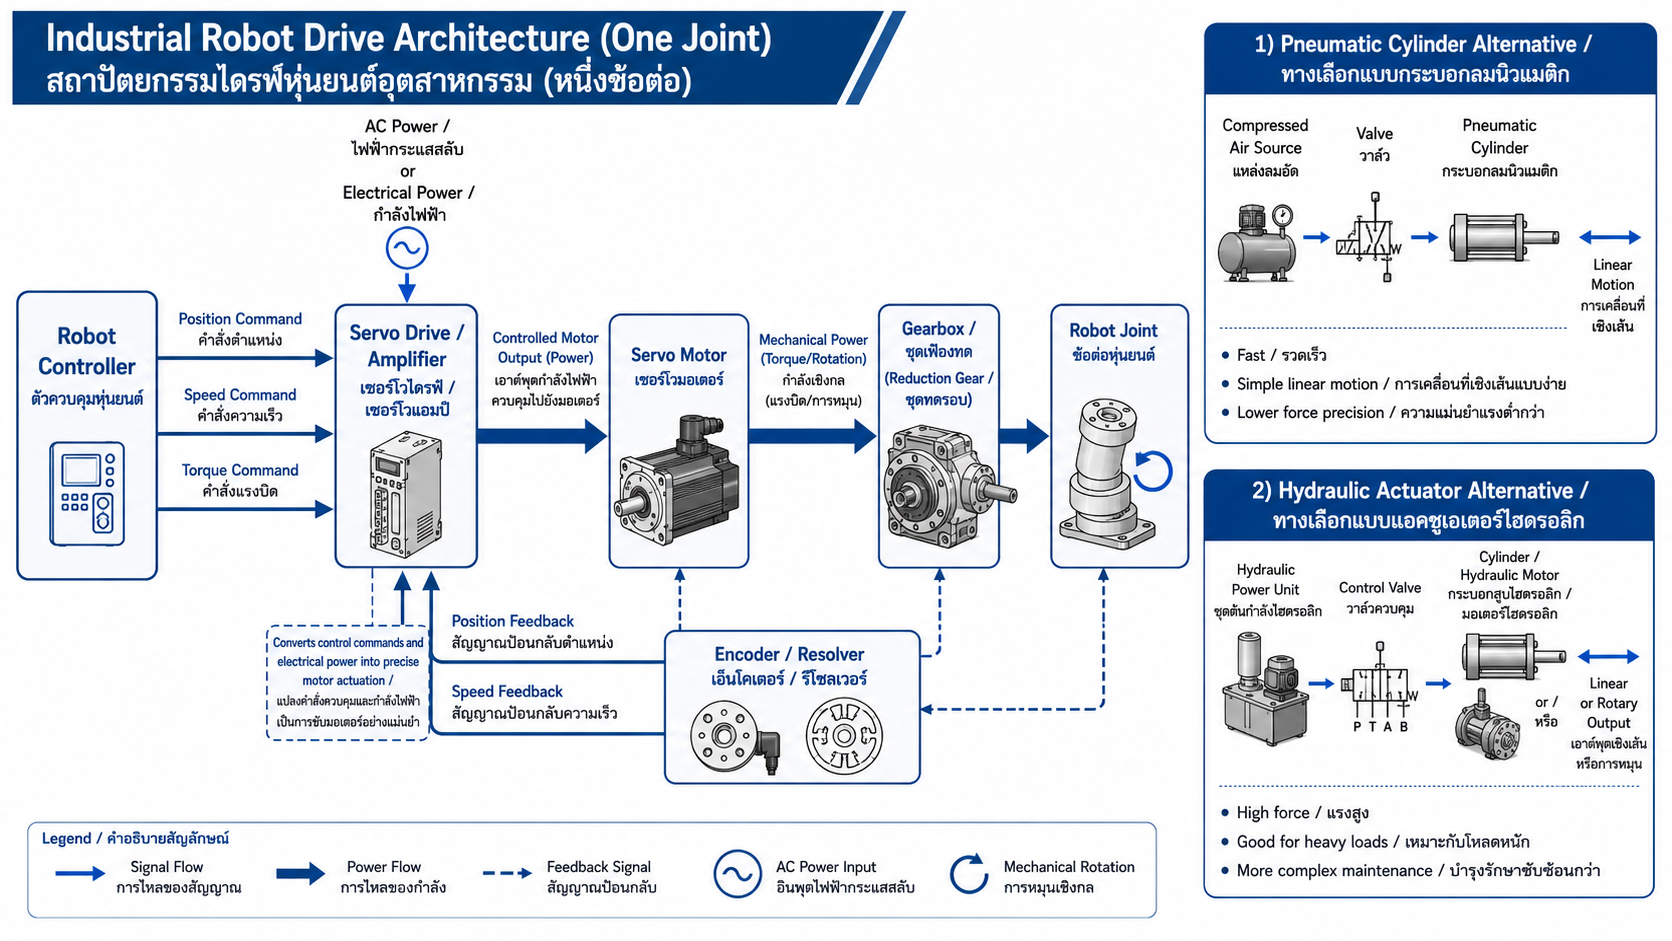
\includegraphics[width=0.8\textwidth]{images/chapter5/figure-1.png}
    \caption{ภาพรวมระบบขับเคลื่อนหุ่นยนต์อุตสาหกรรม}
\end{figure}

\par\noindent\rule{\textwidth}{0.4pt}\par

\subsection{บทนำ}

หุ่นยนต์อุตสาหกรรมต้องเคลื่อนที่ตามวิถีที่กำหนดภายใต้โหลดที่เปลี่ยนแปลง ความเร็วสูง และข้อจำกัดด้านความปลอดภัย ตัวอย่างเช่น หุ่นยนต์เชื่อมต้องรักษาความเร็วปลายหัวเชื่อมให้สม่ำเสมอ หุ่นยนต์หยิบวางต้องหยุดตรงตำแหน่งโดยไม่สั่น หุ่นยนต์พ่นสีต้องเคลื่อนที่ราบรื่น ส่วนหุ่นยนต์จัดเรียงพาเลตต้องสร้างแรงบิดเพียงพอเมื่อตำแหน่งแขนยื่นออกไกล การออกแบบระบบขับเคลื่อนจึงต้องตอบคำถามอย่างน้อยสี่ประการ ได้แก่ ต้องการแรงหรือแรงบิดเท่าใด ต้องการความเร็วและความเร่งเท่าใด ต้องการความละเอียดและความสามารถทำซ้ำระดับใด และควรใช้พลังงาน ตัวกระทำ ตัวตรวจจับ และวิธีควบคุมแบบใด

คำว่า \textbf{Servo Drive} และ \textbf{Servo Amplifier} มักใช้แทนกันในงานอุตสาหกรรม อย่างไรก็ตาม ในเชิงหน้าที่ Servo Amplifier เน้นส่วนที่ขยายกำลังจากสัญญาณควบคุมไปสู่กระแสและแรงดันสำหรับมอเตอร์ ส่วน Servo Drive มักครอบคลุมกว้างกว่า โดยรวมวงจรแปลงกำลัง ตัวประมวลผลควบคุม อินเทอร์เฟซตัวตรวจจับ การสื่อสาร การป้องกัน และฟังก์ชันความปลอดภัยไว้ในหน่วยเดียว

มาตรฐาน ISO 10218-1:2025 และ ISO 10218-2:2025 เป็นมาตรฐานความปลอดภัยสำคัญสำหรับหุ่นยนต์อุตสาหกรรมและการประยุกต์ใช้ในเซลล์หุ่นยนต์ [1], [2] แม้บทนี้มุ่งเน้นระบบขับเคลื่อน นักศึกษาต้องตระหนักว่าแกนเซอร์โวสามารถสร้างการเคลื่อนที่อย่างรวดเร็วและแรงบิดสูง การทดลองกับ Servo Drive จริงจึงต้องใช้ชุดฝึกที่มีฝาครอบ อุปกรณ์หยุดฉุกเฉิน การจำกัดความเร็ว และการเดินสายกำลังโดยผู้สอนหรือช่างผู้รับผิดชอบเท่านั้น

\par\noindent\rule{\textwidth}{0.4pt}\par

\subsection{เนื้อหาหลัก}

\subsubsection{โครงสร้างของระบบขับเคลื่อนหุ่นยนต์}

ระบบขับเคลื่อนหนึ่งแกนประกอบด้วยแหล่งพลังงาน อุปกรณ์แปลงและควบคุมกำลัง ตัวกระทำ ชุดส่งกำลัง โหลด ตัวตรวจจับ ตัวควบคุม และระบบความปลอดภัย พลังงานไหลจากแหล่งจ่ายผ่าน Drive ไปยังมอเตอร์ ขณะที่ข้อมูลคำสั่งไหลจาก Controller ไปยัง Drive และข้อมูลป้อนกลับไหลจากตัวตรวจจับกลับมายัง Drive หรือ Controller การแยกเส้นทางพลังงานและเส้นทางสัญญาณช่วยให้วิเคราะห์ปัญหาได้ง่ายขึ้น เช่น มอเตอร์ไม่หมุนอาจเกิดจากไฟกำลังไม่พร้อม คำสั่งไม่เข้ามา สัญญาณ Enable ไม่ทำงาน Feedback ผิดปกติ หรือวงจรความปลอดภัยตัดการสร้างแรงบิด

% [รูปที่ 2: เส้นทางพลังงานและเส้นทางสัญญาณของแกนหุ่นยนต์]
% ประเภทภาพ: Block Diagram
% ตำแหน่งที่แนะนำ: หลังหัวข้อ 7.1
% วัตถุประสงค์การเรียนรู้: แยกความแตกต่างระหว่างพลังงาน คำสั่ง และสัญญาณป้อนกลับ
% คำอธิบายภาพ: ใช้ลูกศรหนาสำหรับ Power Flow จาก AC Supply → Rectifier/DC Bus → Inverter → Servo Motor → Gearbox → Joint และลูกศรเส้นบางสำหรับ Signal Flow จาก Robot Controller → Servo Drive รวมถึง Encoder Feedback → Servo Drive และ Safety Chain → Drive Enable/STO
% องค์ประกอบที่ต้องมี: AC Supply, DC Bus, Inverter, Motor, Gearbox, Joint, Controller, Encoder, Safety PLC, STO
% ข้อความหรือป้ายกำกับ: Power Flow, Command Signal, Feedback Signal, Safety Signal
% ภาษาของป้ายกำกับ: ไทยและอังกฤษ
% สัดส่วนภาพ: 16:9
% Image Generation Prompt: Technical block diagram separating power flow and signal flow in an industrial robot servo axis. Thick arrows: AC supply to rectifier and DC bus, inverter, servo motor, gearbox, robot joint. Thin arrows: robot controller command to servo drive, encoder feedback to drive, safety PLC signal to STO and drive enable. Use different line styles rather than relying only on color. Clean engineering textbook style, bilingual Thai-English labels, 16:9.
% Alt Text: แผนภาพแยกเส้นทางไฟกำลัง เส้นทางคำสั่ง เส้นทางป้อนกลับ และเส้นทางความปลอดภัย

\begin{figure}[htbp]
    \centering
    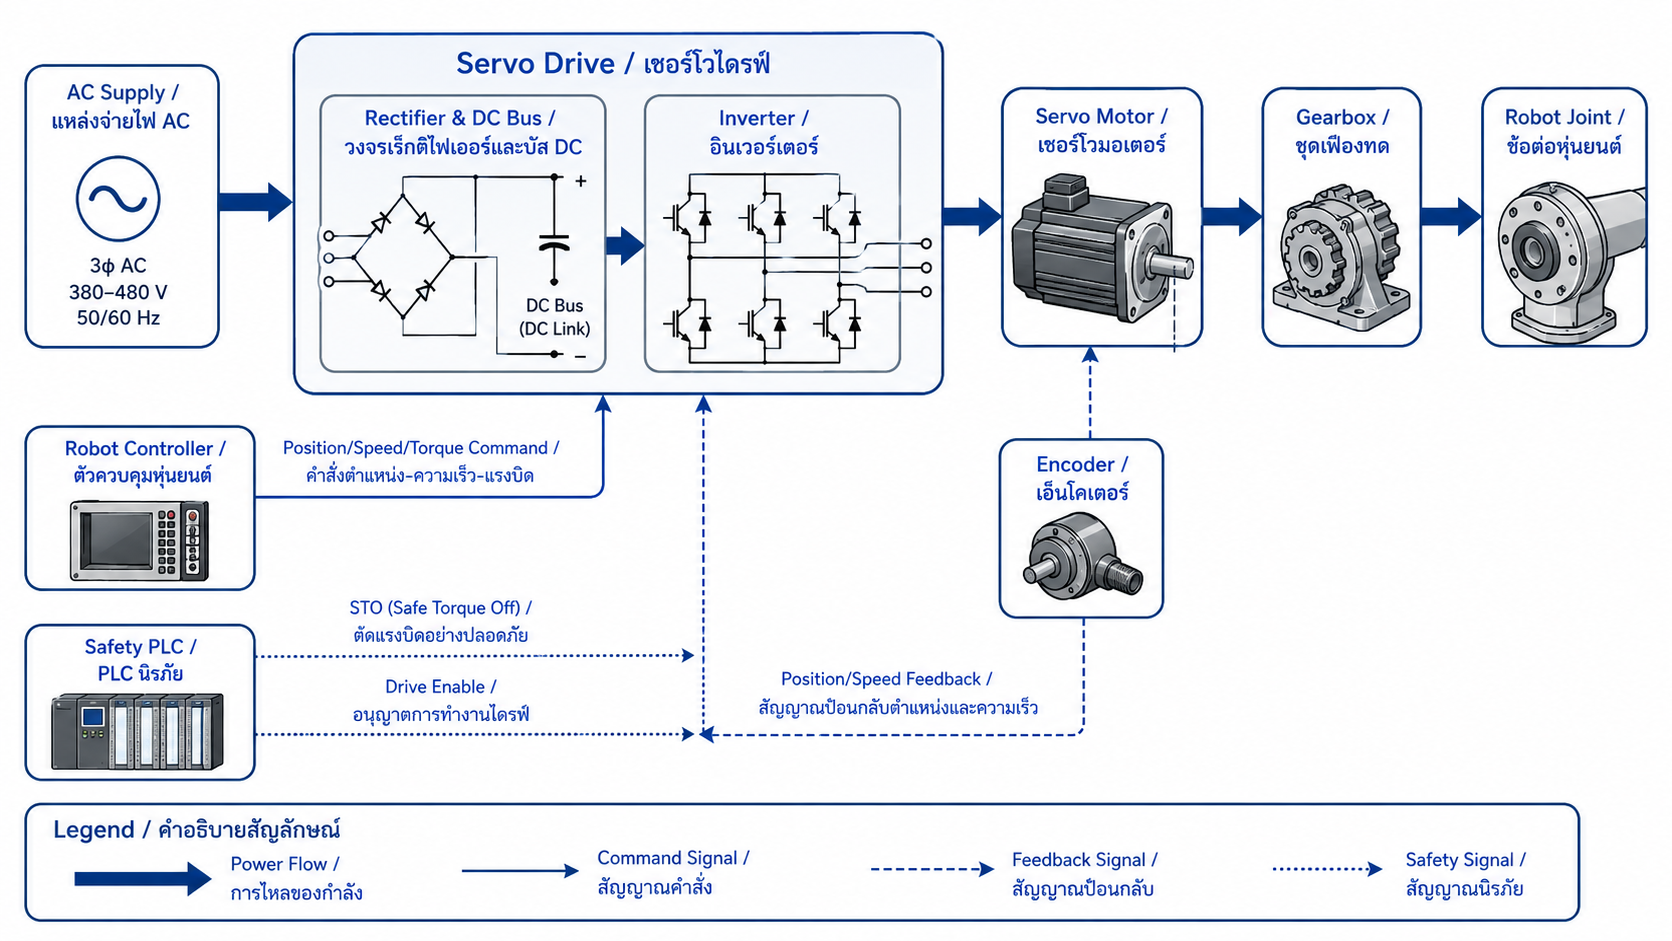
\includegraphics[width=0.8\textwidth]{images/chapter5/figure-2.png}
    \caption{เส้นทางพลังงานและเส้นทางสัญญาณของแกนหุ่นยนต์}
\end{figure}

\subsubsection{การจำแนกระบบขับเคลื่อนตามแหล่งพลังงาน}

\paragraph{ระบบขับเคลื่อนด้วยไฟฟ้า}

ระบบไฟฟ้าใช้มอเตอร์เป็นตัวกระทำและใช้อุปกรณ์อิเล็กทรอนิกส์กำลังควบคุมแรงดัน กระแส ความถี่ และเฟส จุดเด่นคือควบคุมได้ละเอียด เชื่อมต่อกับระบบดิจิทัลได้ง่าย มีประสิทธิภาพดี และรักษาความสะอาดของพื้นที่ผลิตได้ง่ายกว่าระบบของไหล จึงพบมากในหุ่นยนต์เชื่อม หุ่นยนต์ประกอบ หุ่นยนต์หยิบวาง และหุ่นยนต์พ่นสีรุ่นใหม่

ข้อจำกัดสำคัญคือมอเตอร์และ Drive มีขีดจำกัดทางความร้อน ต้องเลือกกำลังและอัตราทดให้เหมาะสม การเปลี่ยนโหลดหรือเกิดการชนอาจทำให้กระแสสูงและเกิด Fault นอกจากนี้สัญญาณ PWM จาก Inverter ก่อให้เกิดสัญญาณรบกวนทางแม่เหล็กไฟฟ้า จึงต้องเดินสายกำลังและสาย Feedback ตามคู่มือผู้ผลิต

\paragraph{ระบบขับเคลื่อนด้วยนิวเมติก}

ระบบนิวเมติกใช้ลมอัดขับกระบอกสูบหรือมอเตอร์ลม Festo อธิบายว่าตัวขับนิวเมติกเปลี่ยนพลังงานความดันเป็นพลังงานการเคลื่อนที่และถ่ายทอดแรง [5] ระบบนี้เหมาะกับการยืด–หด การหนีบ การปล่อยชิ้นงาน หรือกลไกสองตำแหน่ง เนื่องจากโครงสร้างไม่ซับซ้อน น้ำหนักเบา ต้นทุนไม่สูง และให้ความเร็วตอบสนองดี

อย่างไรก็ตาม ลมอัดมีความยืดหยุ่นหรืออัดตัวได้ ทำให้การควบคุมตำแหน่งกึ่งกลางและความแข็งของระบบต่ำกว่าระบบไฟฟ้าหรือไฮดรอลิก การรั่วของลมยังทำให้สิ้นเปลืองพลังงาน และแรงที่ได้จริงต่ำกว่าค่าทฤษฎีเนื่องจากแรงเสียดทานและความดันตกคร่อม

\paragraph{ระบบขับเคลื่อนด้วยไฮดรอลิก}

ระบบไฮดรอลิกใช้น้ำมันหรือของไหลภายใต้ความดันขับกระบอกสูบหรือมอเตอร์ไฮดรอลิก มีความหนาแน่นกำลังสูงและเหมาะกับงานหนัก เช่น หุ่นยนต์หล่อโลหะ งานจับยึดชิ้นงานขนาดใหญ่ หรือระบบเคลื่อนย้ายที่ต้องการแรงมาก ข้อจำกัดคือระบบปั๊ม ถังพัก วาล์ว และท่อต้องได้รับการดูแลอย่างดี การรั่วซึมอาจปนเปื้อนพื้นที่ผลิต อุณหภูมิและความหนืดของของไหลมีผลต่อการตอบสนอง และระบบโดยรวมมีขนาดใหญ่กว่าระบบไฟฟ้า

\newpage

\paragraph{ตารางเปรียบเทียบ}

\begin{table}[htbp]
    \centering
    \begin{tabular}{l l l l}
        \hline
        \textbf{เกณฑ์} & \textbf{ไฟฟ้า} & \textbf{นิวเมติก} & \textbf{ไฮดรอลิก} \\
        \hline
        แหล่งพลังงาน & ไฟฟ้า & ลมอัด & ของไหลแรงดัน \\
        ความแม่นยำตำแหน่ง & สูงเมื่อใช้ Servo + Feedback & ต่ำถึงปานกลาง & ปานกลางถึงสูงเมื่อใช้วาล์วเซอร์โวและ Feedback \\
        ความหนาแน่นกำลัง & ปานกลางถึงสูง & ต่ำถึงปานกลาง & สูงมาก \\
        ความเร็วตอบสนอง & สูง & สูงในงานช่วงชักสั้น & ปานกลางถึงสูง \\
        ความแข็งของระบบ & สูง & ต่ำกว่าเพราะลมอัดตัวได้ & สูง \\
        ความสะอาด & ดี & ดีถ้าคุณภาพลมเหมาะสม & ต้องควบคุมการรั่วซึม \\
        การบำรุงรักษา & ปานกลาง & ปานกลาง & สูง \\
        งานเด่น & แกนหุ่นยนต์ทั่วไป & Gripper, Stopper, Ejector & งานแรงสูง งานหนัก \\
        การควบคุมต่อเนื่อง & ทำได้ดี & ทำได้แต่ซับซ้อน & ทำได้ด้วยวาล์วสัดส่วนหรือวาล์วเซอร์โว \\
        ความเสี่ยงหลัก & ไฟฟ้า การหมุนฉับพลัน ความร้อน & ลมค้าง การดีดตัว เสียง & แรงดันสูง การรั่ว การฉีดของไหล \\
        \hline
    \end{tabular}
\end{table}

% [รูปที่ 3: เปรียบเทียบระบบขับเคลื่อนไฟฟ้า นิวเมติก และไฮดรอลิก]
% ประเภทภาพ: Technical Illustration / Infographic
% ตำแหน่งที่แนะนำ: หลังหัวข้อ 7.2.4
% วัตถุประสงค์การเรียนรู้: ช่วยเลือกชนิดระบบขับเคลื่อนตามลักษณะงาน
% คำอธิบายภาพ: แสดงสามคอลัมน์ ได้แก่ Electric Servo Axis, Pneumatic Gripper และ Hydraulic Heavy-Duty Joint พร้อมไอคอนพลังงาน ตัวกระทำ ช่วงแรง ความแม่นยำ การบำรุงรักษา และตัวอย่างงาน
% องค์ประกอบที่ต้องมี: Servo motor and drive, pneumatic cylinder and valve, hydraulic cylinder and pump, comparison scales
% ข้อความหรือป้ายกำกับ: Precision, Force Density, Maintenance, Typical Use
% ภาษาของป้ายกำกับ: ไทยและอังกฤษ
% สัดส่วนภาพ: 16:9
% Image Generation Prompt: Educational three-column comparison of industrial robot drive systems: electric servo axis, pneumatic gripper actuator, and hydraulic heavy-duty joint. Show energy source, actuator, typical force capability, positioning precision, maintenance level, and representative robot application. Clean engineering textbook infographic, technically accurate, bilingual Thai-English labels, 16:9.
% Alt Text: อินโฟกราฟิกเปรียบเทียบข้อเด่น ข้อจำกัด และงานเหมาะสมของระบบไฟฟ้า นิวเมติก และไฮดรอลิก

\begin{figure}[htbp]
    \centering
    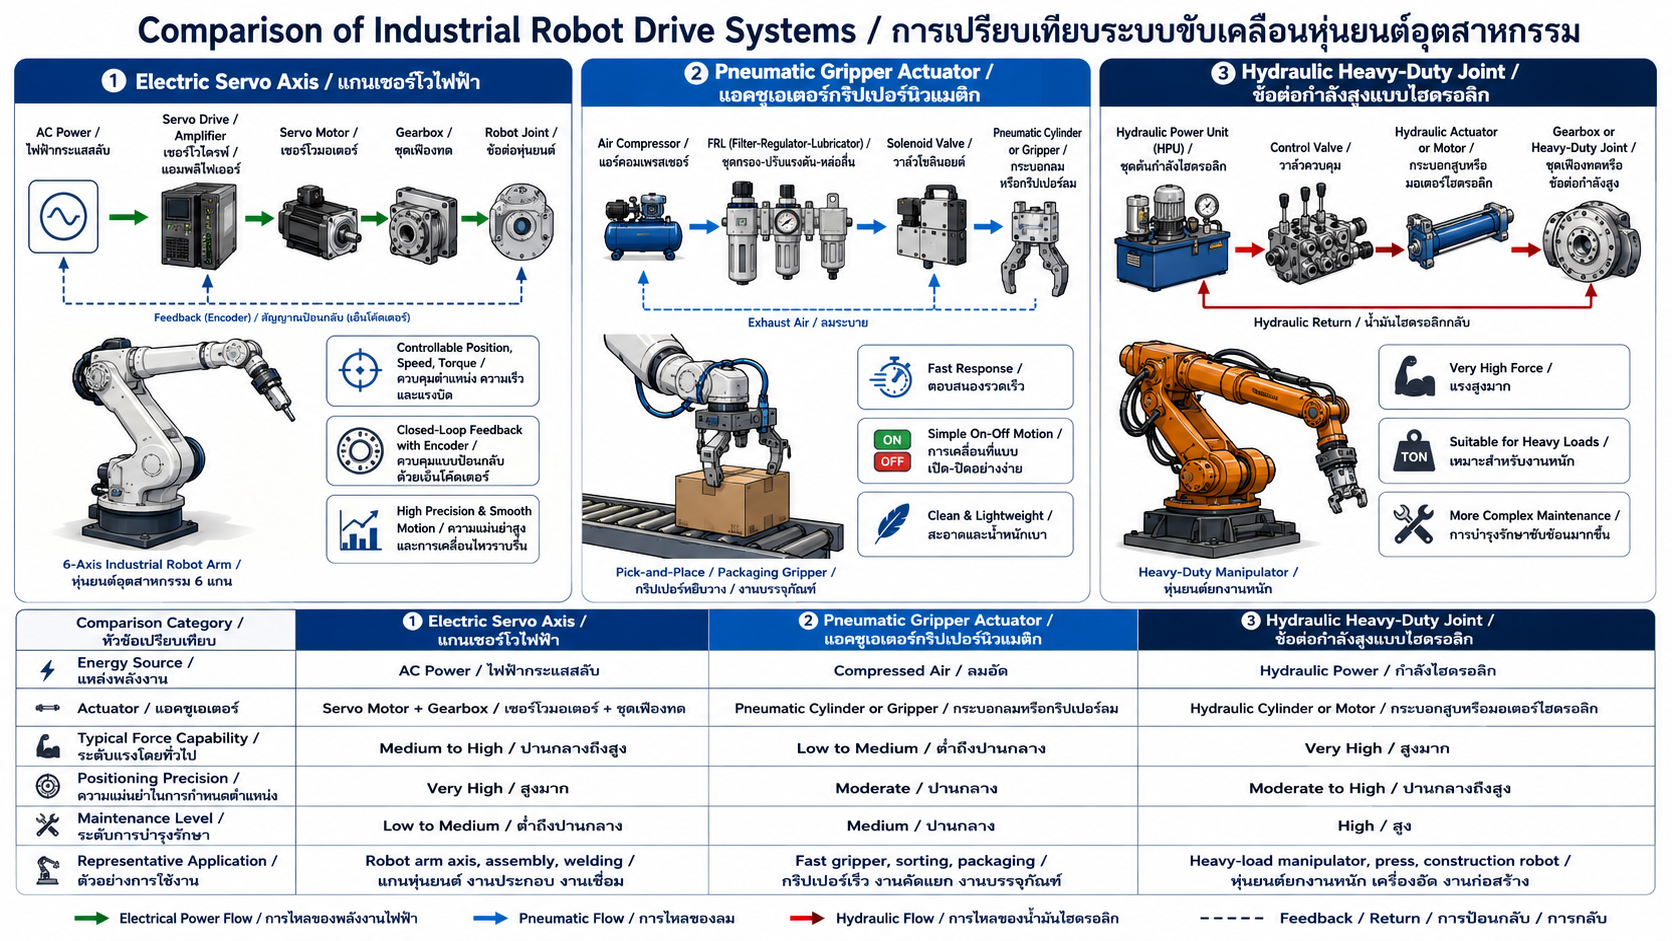
\includegraphics[width=0.8\textwidth]{images/chapter5/figure-3.png}
    \caption{เปรียบเทียบระบบขับเคลื่อนไฟฟ้า นิวเมติก และไฮดรอลิก}
\end{figure}

\subsubsection{มอเตอร์กระแสตรง}

มอเตอร์กระแสตรง (DC Motor) เปลี่ยนพลังงานไฟฟ้ากระแสตรงเป็นแรงบิดทางกล มอเตอร์แบบแปรงถ่านมีคอมมิวเตเตอร์และแปรงถ่านช่วยสลับทิศกระแสในขดลวด ข้อดีคือแบบจำลองและการควบคุมพื้นฐานเข้าใจง่าย แต่แปรงถ่านสึกหรอและเกิดประกายไฟ มอเตอร์ DC แบบไร้แปรงถ่านหรือ BLDC ใช้วงจรอิเล็กทรอนิกส์สลับเฟสแทน จึงมีอายุใช้งานสูงและเหมาะกับงานอัตโนมัติ

\paragraph{แบบจำลองทางไฟฟ้า}

สำหรับมอเตอร์ DC แบบควบคุมแรงดันอาร์มาเจอร์ สมการวงจรคือ

\[
V_a(t)=L_a\frac{di_a(t)}{dt}+R_a i_a(t)+e_b(t)
\]

โดยที่

\begin{itemize}
    \item $V_a$ คือแรงดันอาร์มาเจอร์ หน่วยโวลต์
    \item $L_a$ คือความเหนี่ยวนำอาร์มาเจอร์ หน่วยเฮนรี
    \item $R_a$ คือความต้านทานอาร์มาเจอร์ หน่วยโอห์ม
    \item $i_a$ คือกระแสอาร์มาเจอร์ หน่วยแอมแปร์
    \item $e_b$ คือแรงเคลื่อนไฟฟ้าย้อนกลับ หน่วยโวลต์
\end{itemize}

แรงเคลื่อนไฟฟ้าย้อนกลับแปรผันกับความเร็วเชิงมุม

\[
e_b(t)=K_e\omega(t)
\]

แรงบิดแม่เหล็กไฟฟ้าแปรผันกับกระแส

\[
T_m(t)=K_t i_a(t)
\]

โดย $K_e$ คือค่าคงที่ Back EMF และ $K_t$ คือค่าคงที่แรงบิด สำหรับหน่วย SI ค่าตัวเลขของสองค่าคงที่อาจเท่ากันเมื่อใช้หน่วยที่สอดคล้องกัน แต่ต้องตรวจสอบนิยามจาก Data Sheet เสมอ แบบจำลองของ MathWorks ใช้ความสัมพันธ์ทางไฟฟ้าและแรงบิดในลักษณะเดียวกัน [8]

\paragraph{แบบจำลองทางกล}

สมการสมดุลแรงบิดของเพลามอเตอร์คือ

\[
J\frac{d\omega(t)}{dt}+B\omega(t)+T_L(t)=T_m(t)
\]

โดย

\begin{itemize}
    \item $J$ คือโมเมนต์ความเฉื่อยรวมที่เพลามอเตอร์ หน่วย $\text{kg·m}^2$
    \item $B$ คือสัมประสิทธิ์แรงเสียดทานเชิงหนืด หน่วย $\text{N·m·s/rad}$
    \item $T_L$ คือแรงบิดโหลด หน่วย $\text{N·m}$
    \item $\omega$ คือความเร็วเชิงมุม หน่วย $\text{rad/s}$
\end{itemize}

ตำแหน่งเชิงมุมสัมพันธ์กับความเร็วตาม

\[
\frac{d\theta(t)}{dt}=\omega(t)
\]

เมื่อแปลงลาปลาซและสมมติค่าเริ่มต้นเป็นศูนย์ ฟังก์ชันถ่ายโอนจากแรงดันไปยังความเร็วคือ

\[
\frac{\Omega(s)}{V_a(s)}
=
\frac{K_t}
{(L_as+R_a)(Js+B)+K_eK_t}
\]

และจากแรงดันไปยังตำแหน่งคือ

\[
\frac{\Theta(s)}{V_a(s)}
=
\frac{K_t}
{s\left[(L_as+R_a)(Js+B)+K_eK_t\right]}
\]

\textbf{สมมติฐานและข้อจำกัด}

\begin{enumerate}
    \item สนามแม่เหล็กอยู่ในช่วงเชิงเส้นและไม่อิ่มตัว
    \item ค่าพารามิเตอร์คงที่
    \item ไม่รวม Dead Zone แรงเสียดทานคูลอมบ์ และความไม่เชิงเส้นของแปรงถ่าน
    \item ชุดส่งกำลังไม่มี Backlash ในแบบจำลองพื้นฐาน
\end{enumerate}

% [รูปที่ 4: แบบจำลองไฟฟ้าและกลไกของมอเตอร์ DC]
% ประเภทภาพ: Technical Illustration / Equivalent Circuit
% ตำแหน่งที่แนะนำ: หลังหัวข้อ 7.3.2
% วัตถุประสงค์การเรียนรู้: เชื่อมโยงแรงดัน กระแส Back EMF แรงบิด ความเร็ว และโหลด
% คำอธิบายภาพ: ด้านซ้ายเป็นวงจร $V_a$, $R_a$, $L_a$, Back EMF $e_b=K_e\omega$ ด้านขวาเป็นเพลาแสดง $T_m=K_ti_a$, inertia $J$, viscous friction $B$, load torque $T_L$ และความเร็ว $\omega$
% องค์ประกอบที่ต้องมี: Voltage source, resistor, inductor, back EMF, motor shaft, inertia, friction, load torque
% ข้อความหรือป้ายกำกับ: Electrical Subsystem, Mechanical Subsystem
% ภาษาของป้ายกำกับ: อังกฤษพร้อมสัญลักษณ์สมการ
% สัดส่วนภาพ: 16:9
% Image Generation Prompt: Clean engineering textbook diagram of an armature-controlled DC motor model. Left side: voltage Va, armature resistance Ra, inductance La, current ia, back EMF eb = Ke omega. Right side: electromagnetic torque Tm = Kt ia driving inertia J and viscous friction B against load torque TL, with angular speed omega and position theta. Clear coupling arrows between electrical and mechanical subsystems, white background, 16:9.
% Alt Text: แบบจำลองมอเตอร์ DC แสดงวงจรอาร์มาเจอร์และสมดุลแรงบิดทางกล

\begin{figure}[htbp]
    \centering
    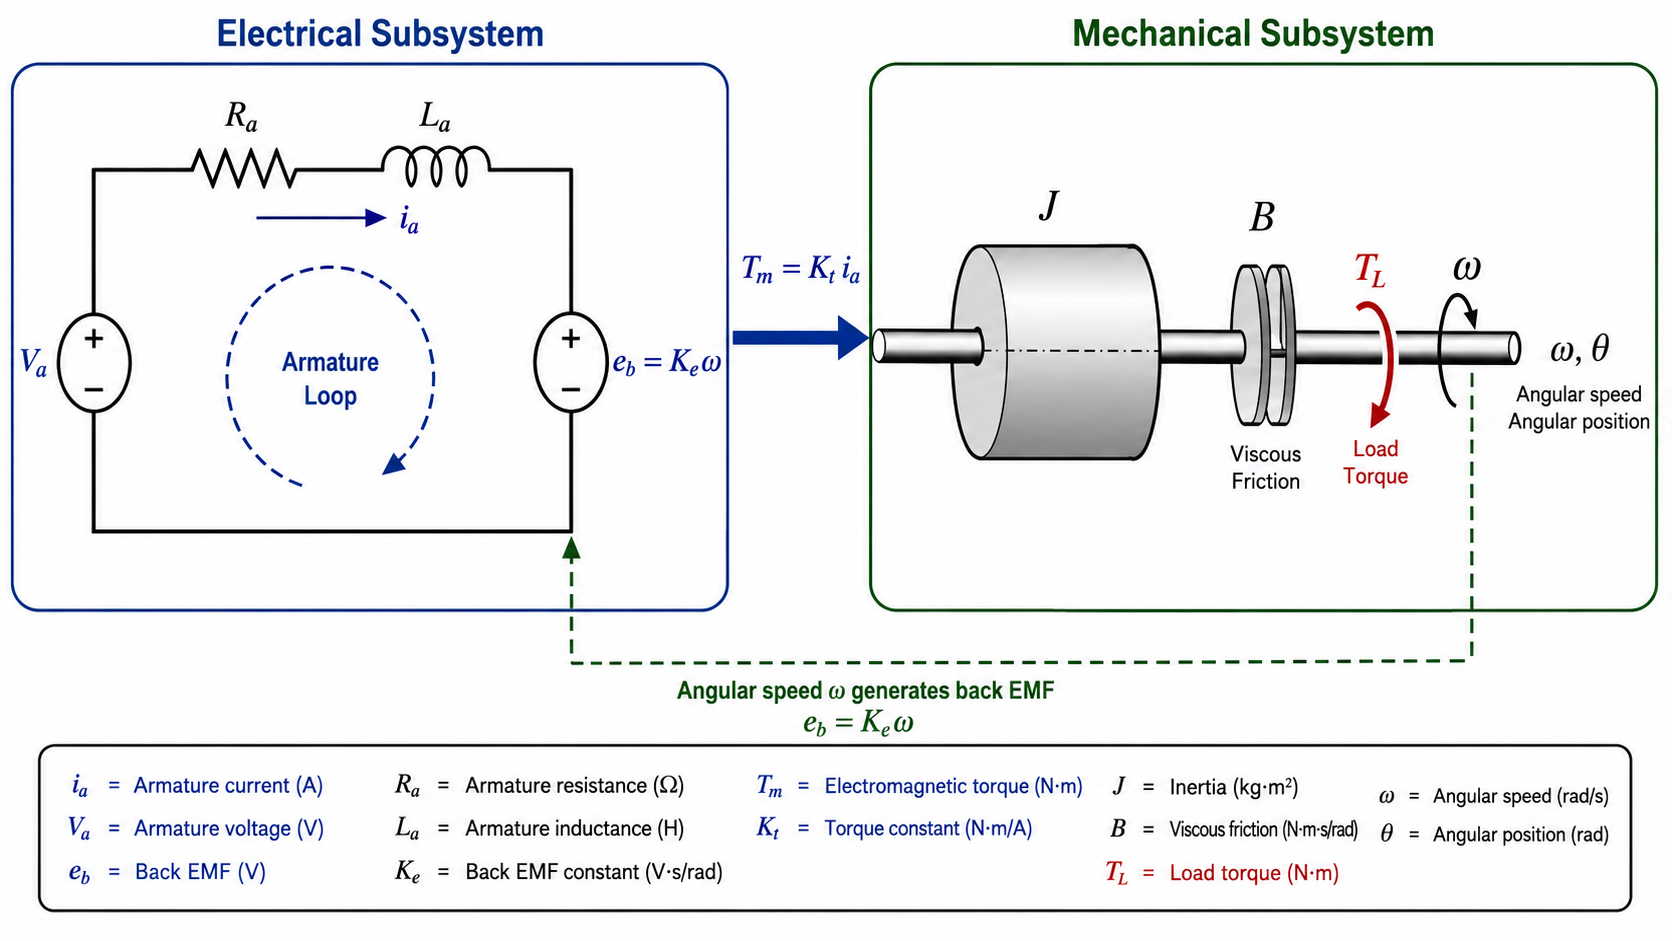
\includegraphics[width=0.8\textwidth]{images/chapter5/figure-4.png}
    \caption{แบบจำลองไฟฟ้าและกลไกของมอเตอร์ DC}
\end{figure}

\paragraph{ตัวอย่างที่ 1 ตัวอย่างเพิ่มเติมเพื่อการเรียนรู้: แรงบิดจากกระแสมอเตอร์ DC}

มอเตอร์มีค่าคงที่แรงบิด $K_t=0.18\ \text{N·m/A}$ และมีกระแสอาร์มาเจอร์ $i_a=6.0\ \text{A}$

\[
T_m=K_ti_a=(0.18)(6.0)=1.08\ \text{N·m}
\]

ดังนั้นมอเตอร์สร้างแรงบิดแม่เหล็กไฟฟ้า \textbf{1.08 N·m} ก่อนหักแรงเสียดทานและการสูญเสีย หากโหลดต้องการ 0.90 N·m ส่วนต่างจะใช้เร่งมวลหมุนและเอาชนะแรงเสียดทาน

\subsubsection{มอเตอร์สเต็ปเปอร์}

มอเตอร์สเต็ปเปอร์ (Stepper Motor) หมุนทีละมุมคงที่ตามลำดับพัลส์คำสั่ง จึงเหมาะกับระบบกำหนดตำแหน่งที่โหลดไม่เปลี่ยนมากและไม่ต้องการตัวตรวจจับป้อนกลับทุกกรณี Oriental Motor อธิบายว่ามอเตอร์สเต็ปเปอร์ควบคุมมุมหมุนและความเร็วได้จากจำนวนและความถี่ของพัลส์ [7]

ชนิดที่พบได้บ่อย ได้แก่ Permanent Magnet, Variable Reluctance และ Hybrid Stepper โดย Hybrid Stepper นิยมในงานอัตโนมัติ มุมก้าวพื้นฐานที่พบทั่วไป เช่น $1.8^\circ$ หรือ $0.9^\circ$ ต่อก้าว

\paragraph{ความสัมพันธ์ของมุมก้าวและจำนวนพัลส์}

ถ้ามุมก้าวพื้นฐานเท่ากับ $\alpha_s$

\[
N_s=\frac{360^\circ}{\alpha_s}
\]

ถ้า Driver ใช้ Microstepping $m$ ไมโครสเต็ปต่อหนึ่ง Full Step

\[
N_p=N_s m
\]

กำหนดอัตราทด

\[
n=\frac{\omega_m}{\omega_L}
\]

จำนวนพัลส์ที่ต้องใช้เพื่อให้โหลดหมุนมุม $\theta_L$ คือ

\[
N_{\text{cmd}}
=
\frac{\theta_L}{360^\circ}
N_smn
\]

ถ้าความถี่พัลส์เท่ากับ $f_p$

\[
N_m=\frac{60f_p}{N_p}
\]

หน่วยรอบต่อนาที

\textbf{ข้อจำกัดของ Stepper แบบวงเปิด}

\begin{itemize}
    \item อาจหลุดก้าวเมื่อแรงบิดโหลดสูงหรือเร่งเร็วเกินไป
    \item แรงบิดลดลงเมื่อความเร็วเพิ่ม
    \item อาจเกิดเรโซแนนซ์ในบางช่วงความเร็ว
    \item Microstepping ทำให้การเคลื่อนที่นุ่มขึ้น แต่ไม่ทำให้ Accuracy เพิ่มตามสัดส่วนเสมอ
    \item เมื่อไม่มี Feedback ระบบไม่ทราบว่าตำแหน่งจริงตรงกับจำนวนพัลส์หรือไม่
\end{itemize}

% [รูปที่ 5: หลักการ Full Step, Half Step และ Microstepping]
% ประเภทภาพ: Technical Illustration / Sequence Diagram
% ตำแหน่งที่แนะนำ: หลังหัวข้อ 7.4.1
% วัตถุประสงค์การเรียนรู้: แสดงความสัมพันธ์ระหว่างลำดับกระแสเฟสและมุมโรเตอร์
% คำอธิบายภาพ: แสดงสเตเตอร์สองเฟส โรเตอร์แม่เหล็ก และตำแหน่งโรเตอร์สำหรับ Full Step, Half Step และ Microstepping พร้อมกราฟกระแสเฟส A และ B แบบไซน์–โคไซน์
% องค์ประกอบที่ต้องมี: Phase A, Phase B, rotor, step angle, current waveforms, pulse sequence
% ข้อความหรือป้ายกำกับ: Full Step, Half Step, Microstep
% ภาษาของป้ายกำกับ: อังกฤษ
% สัดส่วนภาพ: 16:9
% Image Generation Prompt: Educational technical diagram explaining a two-phase hybrid stepper motor. Show rotor positions for full-step, half-step, and microstepping, plus phase-A and phase-B current waveforms with sine-cosine relationship. Clearly indicate step angle and command pulses. White background, engineering textbook style, no decorative effects, 16:9.
% Alt Text: ภาพแสดงการเปลี่ยนตำแหน่งโรเตอร์ของมอเตอร์สเต็ปเปอร์เมื่อใช้ Full Step, Half Step และ Microstepping

\begin{figure}[htbp]
    \centering
    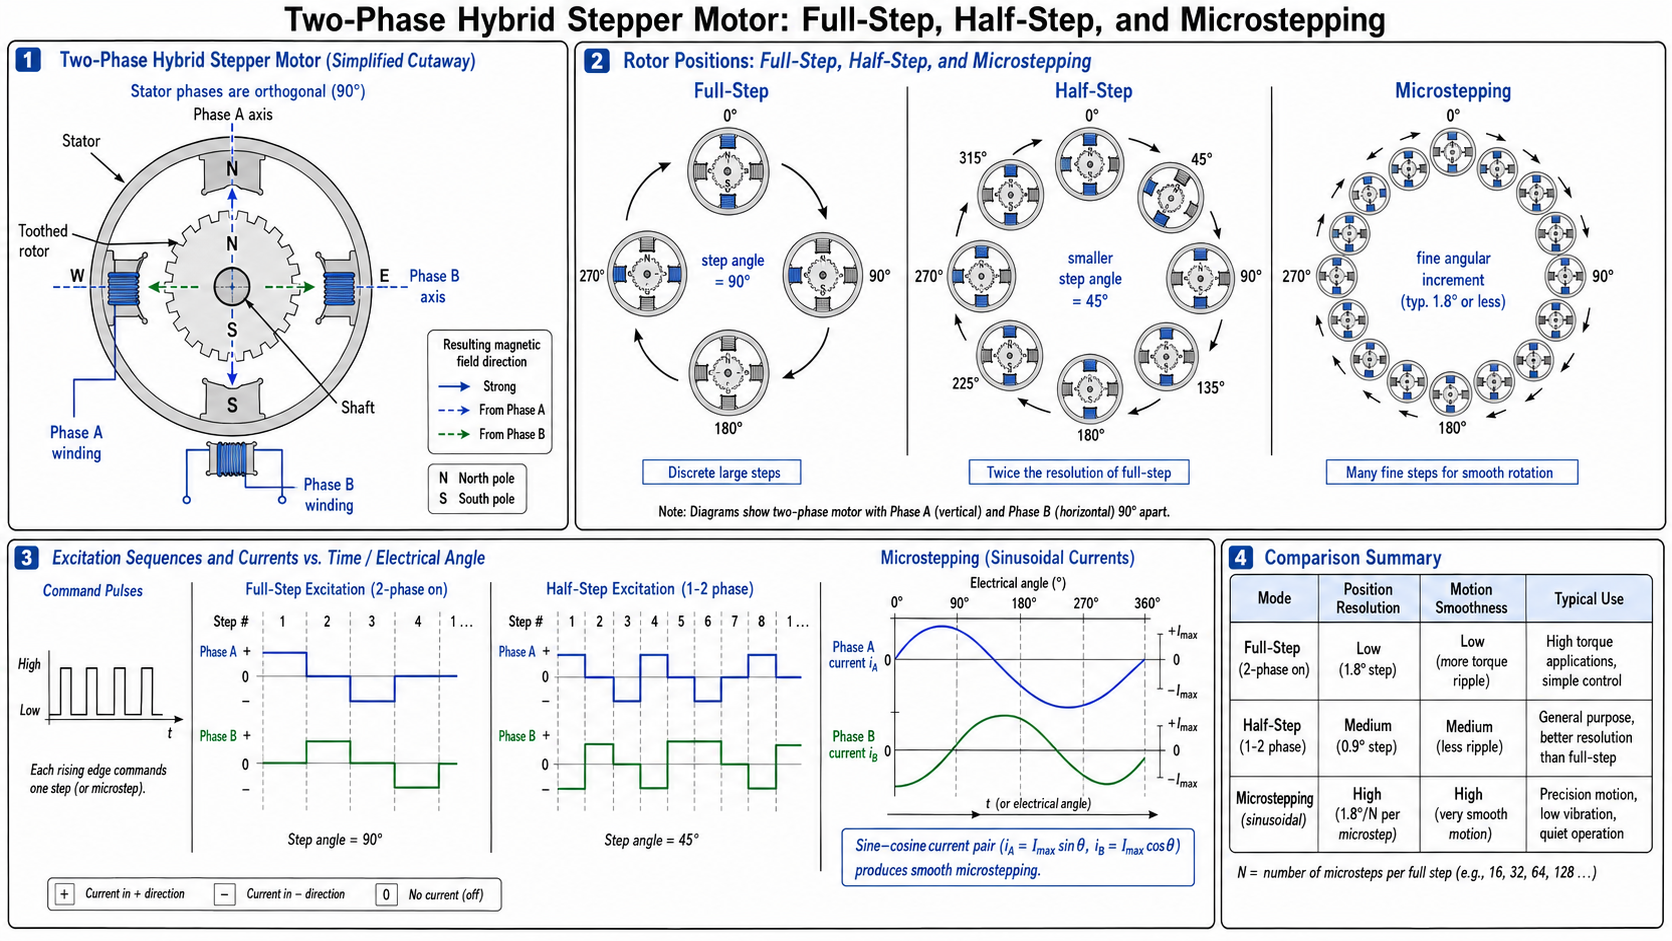
\includegraphics[width=0.8\textwidth]{images/chapter5/figure-5.png}
    \caption{หลักการ Full Step, Half Step และ Microstepping}
\end{figure}

\paragraph{ตัวอย่างที่ 2 ตัวอย่างเพิ่มเติมเพื่อการเรียนรู้: จำนวนพัลส์ของ Stepper พร้อมชุดเกียร์}

มอเตอร์มีมุมก้าว $1.8^\circ$ ใช้ Microstepping 16 และชุดเกียร์ $n=5$ ต้องการให้ด้านโหลดหมุน $90^\circ$

\[
N_s=\frac{360}{1.8}=200
\]

\[
N_p=200(16)=3200\ \text{pulse/rev}
\]

\[
N_{\text{cmd}}
=
\frac{90}{360}(3200)(5)
=
4000\ \text{pulse}
\]

ดังนั้นต้องส่ง \textbf{4,000 พัลส์} โดยสมมติว่าไม่มีการหลุดก้าว Backlash และข้อผิดพลาดของชุดเกียร์

\subsubsection{มอเตอร์เซอร์โว}

Servo Motor ไม่ได้หมายถึงโครงสร้างมอเตอร์ชนิดเดียว แต่หมายถึงมอเตอร์ที่ออกแบบและใช้งานร่วมกับ Feedback และ Servo Drive เพื่อควบคุมการเคลื่อนที่อย่างแม่นยำ ระบบทั่วไปประกอบด้วยมอเตอร์ ตัวตรวจจับตำแหน่ง Drive และสายเชื่อมต่อ [11]

ชนิดที่พบมาก ได้แก่ AC Permanent Magnet Synchronous Servo Motor, Brushless DC Servo Motor, DC Servo Motor แบบแปรงถ่านในระบบรุ่นเก่า และ Linear Servo Motor

\paragraph{คุณลักษณะสำคัญ}

\begin{itemize}
    \item Rated Power และ Rated Speed
    \item Continuous Torque และ Peak Torque
    \item Maximum Speed
    \item Rotor Inertia
    \item Torque Constant
    \item Encoder Resolution
    \item Brake Option
    \item IP Rating และอุณหภูมิใช้งาน
\end{itemize}

กราฟ Torque–Speed แสดงขอบเขตการทำงานต่อเนื่องและช่วง Peak ชั่วขณะ การเลือกมอเตอร์ต้องตรวจสอบทั้งช่วงเร่ง ความเร็วคงที่ และชะลอ

\[
P_m=T\omega
\]

หากความเร็วกำหนดเป็นรอบต่อนาที

\[
\omega=\frac{2\pi N}{60}
\]

% [รูปที่ 6: กราฟแรงบิด–ความเร็วของ Servo Motor]
% ประเภทภาพ: Graph
% ตำแหน่งที่แนะนำ: หลังหัวข้อ 7.5.1
% วัตถุประสงค์การเรียนรู้: แยกขอบเขตแรงบิดต่อเนื่องและแรงบิดสูงสุดชั่วขณะ
% คำอธิบายภาพ: แกนนอนเป็น Speed (r/min) แกนตั้งเป็น Torque (N·m) แสดง Continuous Operating Region, Intermittent/Peak Region, Rated Point, Maximum Speed และเส้นกำลังคงที่
% องค์ประกอบที่ต้องมี: Rated torque, peak torque, rated speed, maximum speed, continuous region, intermittent region
% ข้อความหรือป้ายกำกับ: Continuous Duty, Peak Duty, Rated Point
% ภาษาของป้ายกำกับ: อังกฤษ
% สัดส่วนภาพ: 16:9
% Image Generation Prompt: Engineering textbook torque-speed graph for an industrial AC servo motor. Horizontal axis speed in r/min, vertical axis torque in N·m. Show continuous operating region, intermittent peak torque region, rated point, rated speed, maximum speed, and a constant-power high-speed region. Clean axes, clear legend, white background, 16:9.
% Graph Generation Prompt: Plot a generic illustrative servo torque-speed envelope, not tied to a specific product. Use normalized torque 0–3 pu and speed 0–3 pu. Continuous torque 1 pu to rated speed 1 pu, then decreasing approximately inversely with speed to 0.4 pu at 2.5 pu speed. Peak torque 3 pu at low speed, tapering to 1 pu near maximum speed. Label all regions and state “Illustrative only—refer to manufacturer data.”
% Alt Text: กราฟแรงบิดเทียบความเร็วแสดงพื้นที่ทำงานต่อเนื่องและพื้นที่แรงบิดสูงสุดช่วงสั้น

\begin{figure}[htbp]
    \centering
    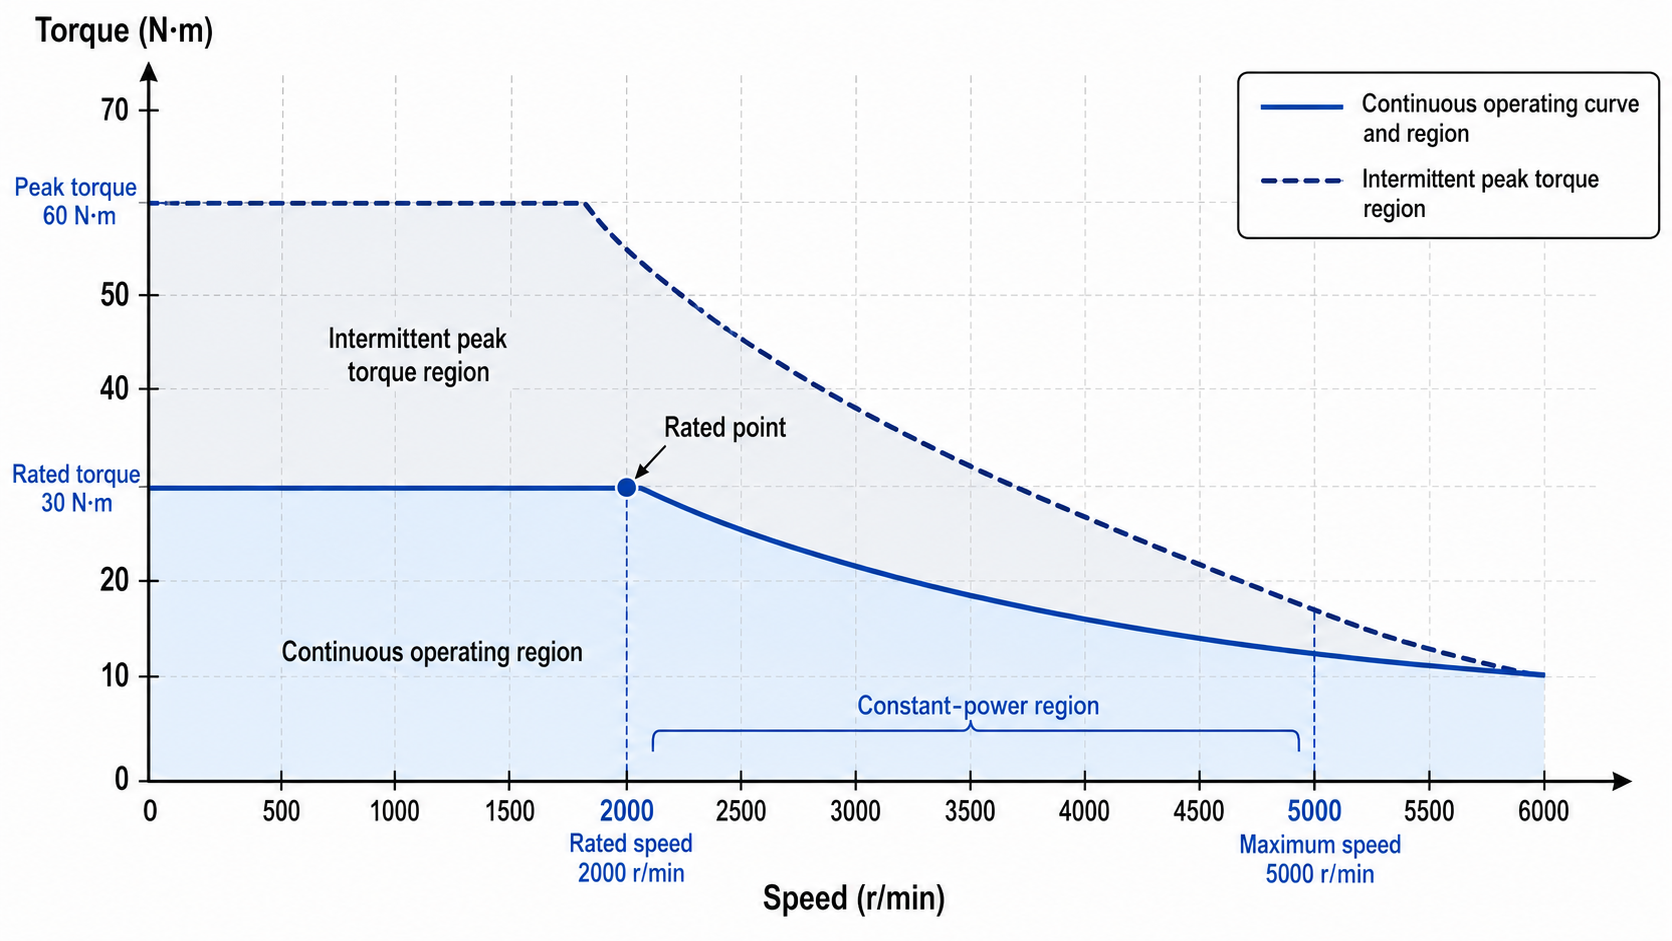
\includegraphics[width=0.8\textwidth]{images/chapter5/figure-6-1.png}
    \caption{กราฟแรงบิด–ความเร็วของ Servo Motor}
\end{figure}

\begin{figure}[htbp]
    \centering
    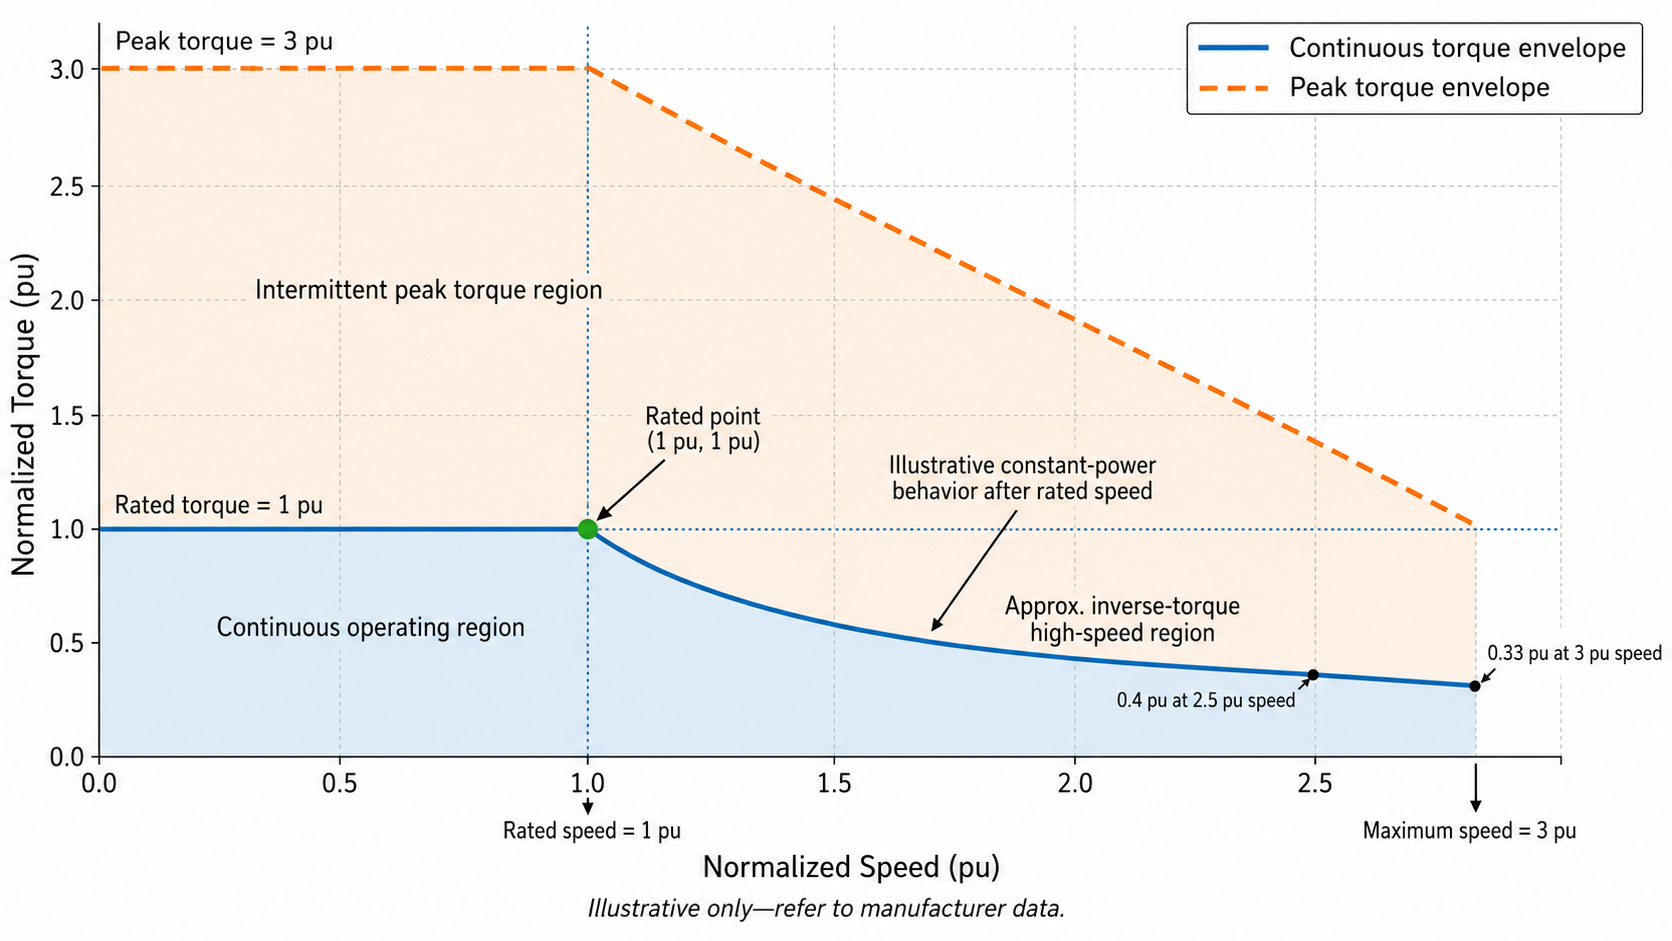
\includegraphics[width=0.8\textwidth]{images/chapter5/figure-6-2.png}
    \caption{กราฟแรงบิด–ความเร็วของ Servo Motor}
\end{figure}

\paragraph{ตัวอย่างที่ 3 ตัวอย่างเพิ่มเติมเพื่อการเรียนรู้: กำลังทางกล}

มอเตอร์สร้างแรงบิด $2.5\ \text{N·m}$ ที่ $1500\ \text{r/min}$

\[
\omega=\frac{2\pi(1500)}{60}=157.08\ \text{rad/s}
\]

\[
P_m=(2.5)(157.08)=392.7\ \text{W}
\]

ดังนั้นกำลังทางกลประมาณ \textbf{393 W} ยังไม่รวมการสูญเสียในมอเตอร์ Drive และชุดเกียร์

\subsubsection{ระบบนิวเมติก}

แรงทฤษฎีของกระบอกสูบคำนวณจาก

\[
F=pA
\]

ด้านยืดของกระบอกสูบสองทาง

\[
A_p=\frac{\pi D^2}{4},
\qquad
F_{\text{ext}}=pA_p
\]

ด้านหด

\[
A_{\text{ann}}=\frac{\pi(D^2-d^2)}{4},
\qquad
F_{\text{ret}}=pA_{\text{ann}}
\]

แรงจริงประมาณได้จาก

\[
F_{\text{actual}}=\eta_p pA-F_f
\]

ความเร็วลูกสูบสัมพันธ์กับอัตราการไหล

\[
Q=Av,
\qquad
v=\frac{Q}{A}
\]

การคำนวณจริงต้องพิจารณาการอัดตัวของลม วาล์ว ท่อ อุณหภูมิ และแรงเสียดทาน คู่มือ Festo แนะนำให้เผื่อแรงจากค่าทฤษฎีและพิจารณาสภาพติดตั้งจริง [6]

\paragraph{ตัวอย่างที่ 4 ตัวอย่างเพิ่มเติมเพื่อการเรียนรู้: แรงยืดของกระบอกลม}

กระบอกลมมี $D=32\ \text{mm}$, $p=6\ \text{bar}$ และ $\eta_p=0.70$

\[
A=\frac{\pi(0.032)^2}{4}=8.042\times10^{-4}\ \text{m}^2
\]

\[
F_{\text{th}}=(6\times10^5)(8.042\times10^{-4})=482.5\ \text{N}
\]

\[
F_{\text{actual}}=0.70(482.5)=337.8\ \text{N}
\]

แรงยืดประมาณ \textbf{338 N}

\subsubsection{ระบบไฮดรอลิก}

ระบบไฮดรอลิกใช้ของไหลที่อัดตัวได้น้อย จึงให้ความแข็งและแรงสูง

\[
F=pA
\]

กำลังไฮดรอลิก

\[
P_h=pQ
\]

กำลังทางกลที่ได้จริง

\[
P_{\text{out}}=\eta_h pQ
\]

\paragraph{ตัวอย่างที่ 5 ตัวอย่างเพิ่มเติมเพื่อการเรียนรู้: แรงจากกระบอกไฮดรอลิก}

$D=40\ \text{mm}$, $p=8\ \text{MPa}$, $\eta_h=0.85$

\[
A=\frac{\pi(0.040)^2}{4}=1.257\times10^{-3}\ \text{m}^2
\]

\[
F_{\text{th}}=(8\times10^6)(1.257\times10^{-3})=10\,053\ \text{N}
\]

\[
F_{\text{actual}}=0.85(10\,053)=8\,545\ \text{N}
\]

ตอบประมาณ \textbf{8.55 kN}

% [รูปที่ 7: วงจรพื้นฐานของระบบนิวเมติกและไฮดรอลิก]
% ประเภทภาพ: Technical Schematic
% ตำแหน่งที่แนะนำ: หลังหัวข้อ 7.7
% วัตถุประสงค์การเรียนรู้: เปรียบเทียบองค์ประกอบและเส้นทางพลังงานของระบบของไหล
% คำอธิบายภาพ: ด้านนิวเมติกแสดง Compressor, FRL, Directional Valve, Flow Control และ Double-Acting Cylinder ด้านไฮดรอลิกแสดง Tank, Pump, Relief Valve, Directional Valve, Flow Control และ Hydraulic Cylinder
% องค์ประกอบที่ต้องมี: Compressor, FRL, pump, tank, relief valve, directional valve, cylinder, pressure and return lines
% ข้อความหรือป้ายกำกับ: Supply, Exhaust, Pressure Line, Return Line
% ภาษาของป้ายกำกับ: อังกฤษ
% สัดส่วนภาพ: 16:9
% Image Generation Prompt: Side-by-side educational fluid power schematics. Left: pneumatic circuit with compressor, air receiver, FRL unit, 5/2 directional valve, flow-control valves, and double-acting cylinder with exhaust. Right: hydraulic circuit with reservoir, pump, pressure relief valve, 4/3 directional valve, flow control, and double-acting hydraulic cylinder with return line. Use standard simplified engineering symbols, clear arrows, white background, 16:9.
% Alt Text: แผนผังเปรียบเทียบวงจรนิวเมติกและไฮดรอลิกสำหรับขับกระบอกสูบสองทาง

\begin{figure}[htbp]
    \centering
    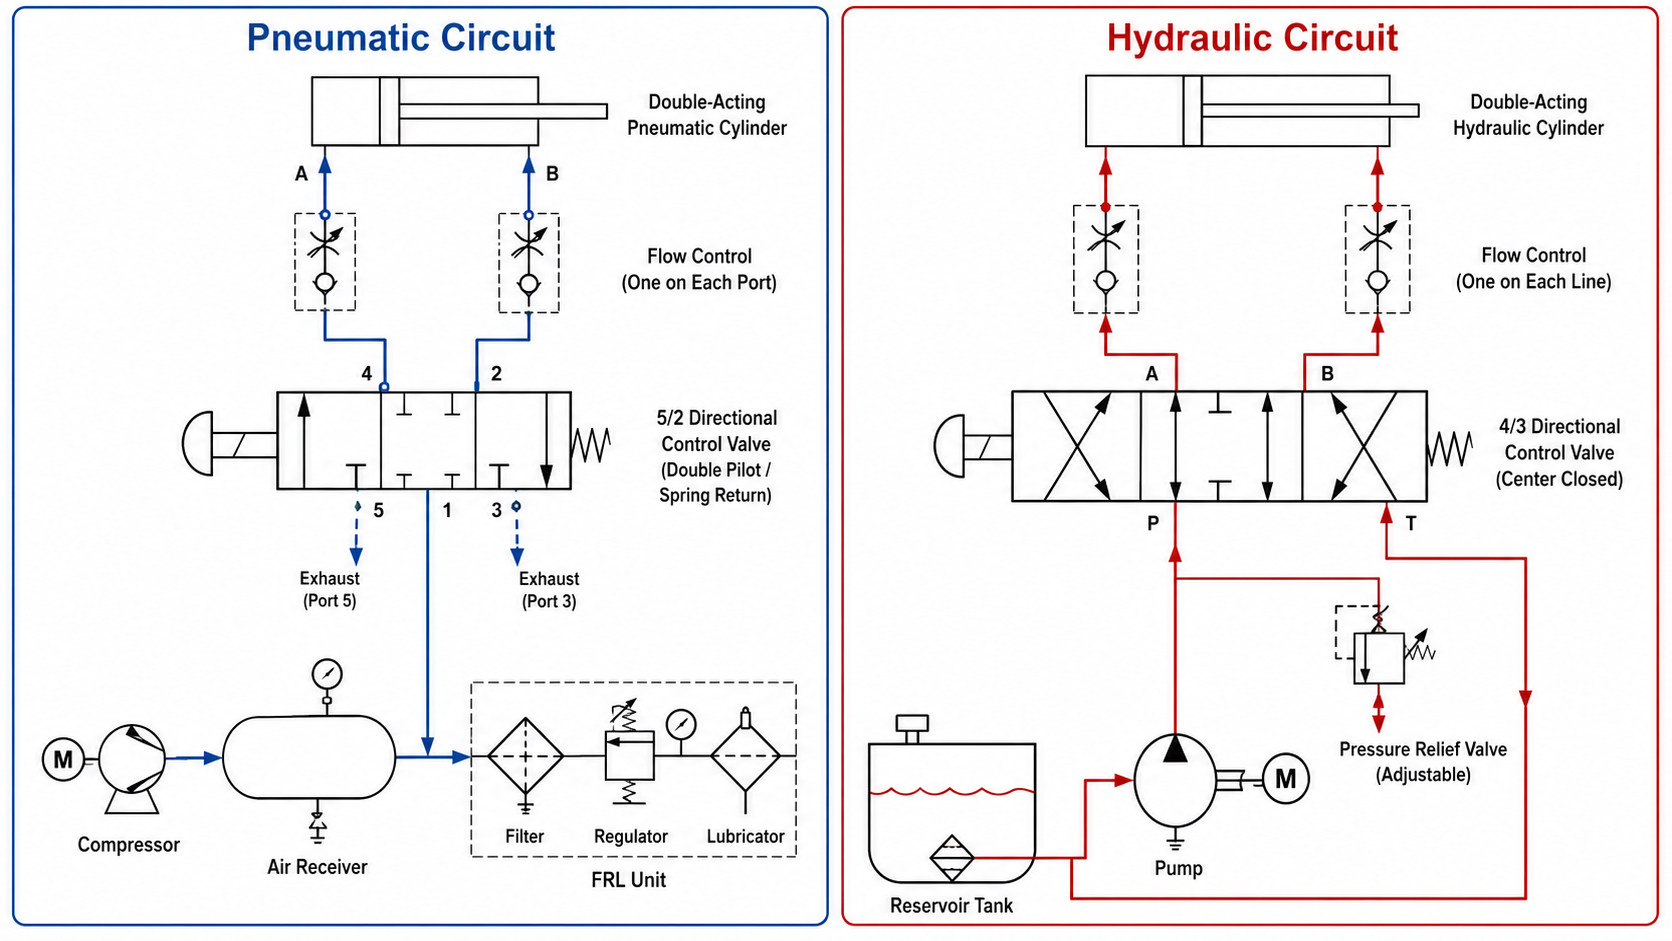
\includegraphics[width=0.8\textwidth]{images/chapter5/figure-7.png}
    \caption{วงจรพื้นฐานของระบบนิวเมติกและไฮดรอลิก}
\end{figure}

\subsubsection{Encoder}

Encoder แปลงตำแหน่งหรือการเคลื่อนที่ทางกลเป็นสัญญาณไฟฟ้า เอกสาร Kollmorgen ระบุว่าคุณภาพของ Feedback มีผลโดยตรงต่อความแม่นยำและการตอบสนองของวงรอบเซอร์โว [4]

\paragraph{Incremental Encoder}

ช่อง A และ B มีเฟสต่างกันประมาณ $90^\circ$ ทางไฟฟ้าเพื่อบอกทิศทาง ช่อง Z ให้หนึ่งพัลส์ต่อรอบสำหรับจุดอ้างอิง หาก Encoder มี $PPR$ และใช้ Quadrature x4

\[
C=4PPR
\]

ตำแหน่งเชิงมุม

\[
\theta=\frac{2\pi N_c}{C}
\]

หรือ

\[
\theta(^\circ)=\frac{360^\circ N_c}{C}
\]

ความเร็วประมาณ

\[
\omega \approx
\frac{2\pi \Delta N_c}{C\Delta t}
\]

\paragraph{Absolute Encoder}

ถ้ามีความละเอียด $b$ บิต

\[
C=2^b
\]

\[
\Delta\theta=\frac{360^\circ}{2^b}
\]

Absolute Encoder แบ่งเป็น Single-turn และ Multi-turn ช่วยลดหรือยกเลิกขั้นตอน Homing ตามสถาปัตยกรรมระบบ ต้องแยก \textbf{Resolution} ออกจาก \textbf{Accuracy, Noise, Bandwidth และ Latency} [4]

\paragraph{ตัวอย่างที่ 6 ตัวอย่างเพิ่มเติมเพื่อการเรียนรู้: Absolute Encoder 20 บิต}

\[
C=2^{20}=1\,048\,576
\]

\[
\Delta\theta=\frac{360^\circ}{1\,048\,576}=0.000343^\circ
\]

1 Count เทียบเท่าประมาณ \textbf{0.000343°} ที่เพลามอเตอร์ แต่ความแม่นยำปลายแขนยังขึ้นกับชุดเกียร์ Backlash ความยืดหยุ่น การสอบเทียบ และโหลด

\subsubsection{Resolver}

Resolver เป็นตัวตรวจจับตำแหน่งเชิงมุมแบบแม่เหล็กไฟฟ้า มีขดลวดกระตุ้นและขดลวดรับสองชุดวางฉากกัน

\[
v_r(t)=V_r\sin(\omega_ct)
\]

\[
v_s(t)=K V_r\sin(\theta)\sin(\omega_ct)
\]

\[
v_c(t)=K V_r\cos(\theta)\sin(\omega_ct)
\]

Resolver-to-Digital Converter หรือ RDC ประมาณมุม $\theta$ จากสัญญาณไซน์และโคไซน์ Resolver ทนความร้อน การสั่น และสภาพแวดล้อมรุนแรง แต่ต้องใช้วงจรกระตุ้นและประมวลผลเฉพาะ [4]

\begin{table}[htbp]
    \centering
    \begin{tabular}{l l l l}
        \hline
        \textbf{เกณฑ์} & \textbf{Incremental Encoder} & \textbf{Absolute Encoder} & \textbf{Resolver} \\
        \hline
        รูปแบบสัญญาณ & พัลส์ A/B/Z & รหัสดิจิทัลหรือ Serial & Sine/Cosine \\
        ตำแหน่งหลังเปิดเครื่อง & ต้อง Homing/อ้างอิง & ทราบตามชนิด & ทราบมุมภายในรอบ \\
        ความละเอียด & ปานกลางถึงสูง & สูงถึงสูงมาก & ขึ้นกับ RDC \\
        ความทนทาน & ปานกลางถึงสูง & ปานกลางถึงสูง & สูงมาก \\
        ความซับซ้อนอินเทอร์เฟซ & ต่ำถึงปานกลาง & ปานกลาง & สูงกว่า \\
        \hline
    \end{tabular}
\end{table}

% [รูปที่ 8: Encoder และ Resolver ในระบบป้อนกลับ]
% ประเภทภาพ: Technical Illustration
% ตำแหน่งที่แนะนำ: หลังหัวข้อ 7.9
% วัตถุประสงค์การเรียนรู้: เปรียบเทียบสัญญาณและหน้าที่ของตัวตรวจจับ
% คำอธิบายภาพ: ซ้ายแสดง Incremental Encoder disk กับสัญญาณ A, B, Z กลางแสดง Absolute Encoder coded disk กับ digital position word ขวาแสดง Resolver กับ excitation, sine output, cosine output และ RDC
% องค์ประกอบที่ต้องมี: A/B/Z waveforms, binary/serial absolute data, resolver excitation, sine/cosine signals, RDC
% ข้อความหรือป้ายกำกับ: Incremental, Absolute, Resolver
% ภาษาของป้ายกำกับ: อังกฤษ
% สัดส่วนภาพ: 16:9
% Image Generation Prompt: Three-panel engineering illustration comparing motor feedback devices. Panel 1: incremental optical encoder with disk and A, B, Z quadrature waveforms. Panel 2: absolute encoder with coded disk and digital position word. Panel 3: resolver with excitation winding, sine and cosine outputs feeding a resolver-to-digital converter. Clear signal arrows, white background, textbook style, 16:9.
% Alt Text: ภาพเปรียบเทียบ Encoder แบบ Incremental, Absolute และ Resolver พร้อมรูปแบบสัญญาณ

\begin{figure}[htbp]
    \centering
    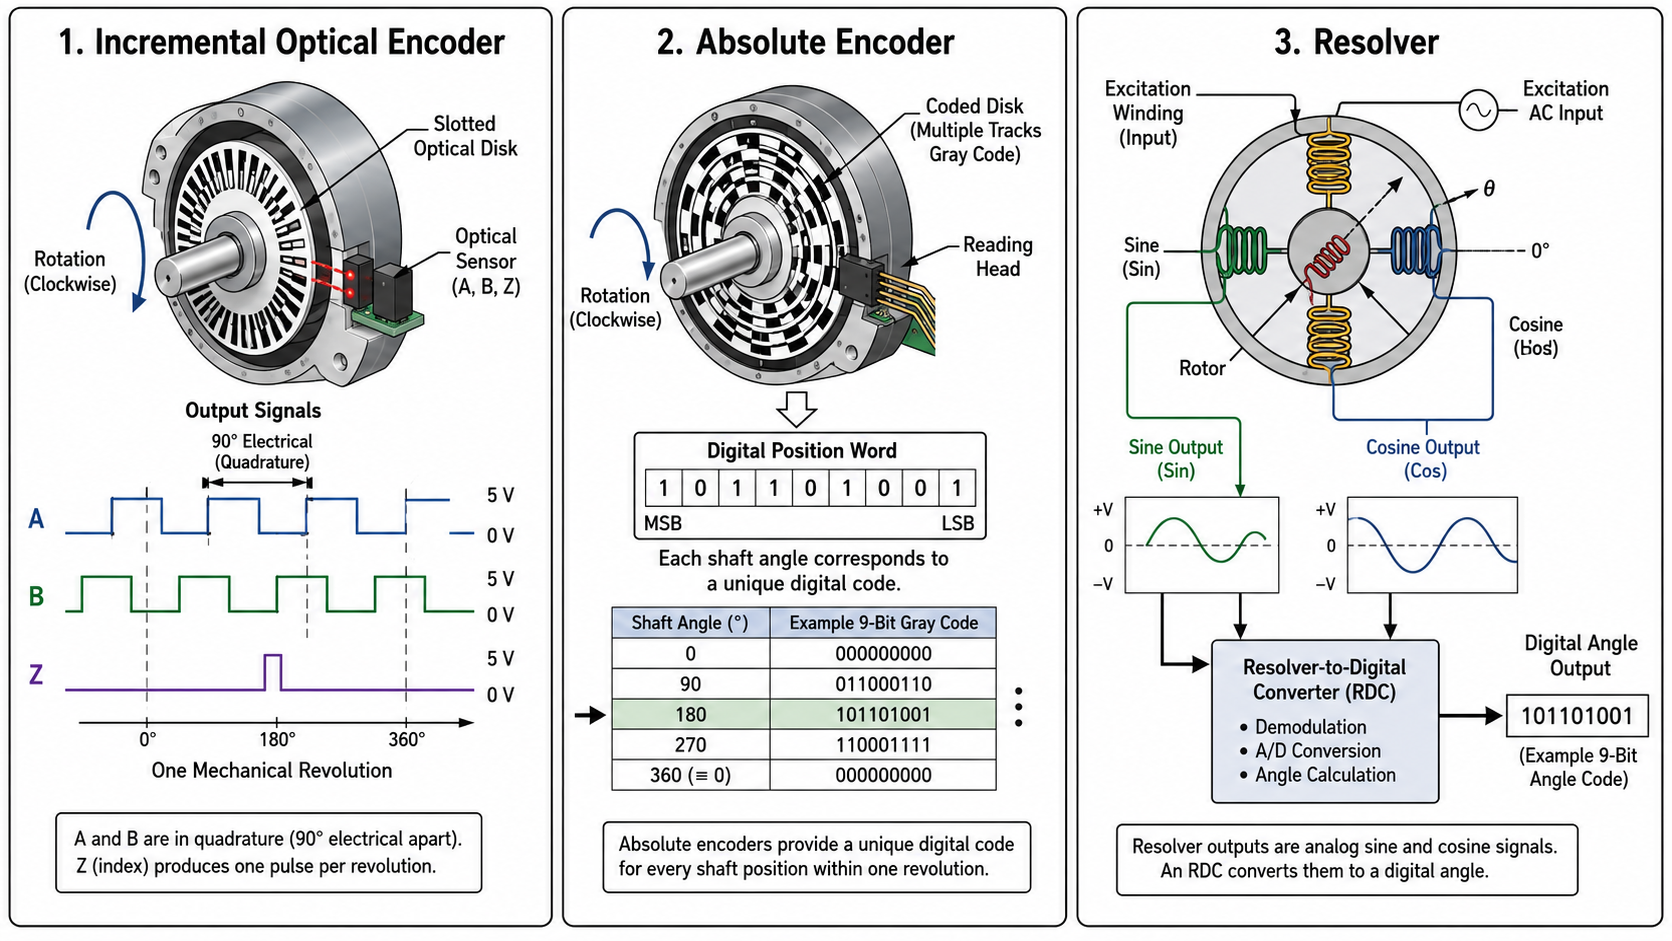
\includegraphics[width=0.8\textwidth]{images/chapter5/figure-8.png}
    \caption{Encoder และ Resolver ในระบบป้อนกลับ}
\end{figure}

\subsubsection{Servo Drive และ Servo Amplifier}

\paragraph{หน้าที่หลัก}

Servo Drive ทำหน้าที่เป็นตัวกลางระหว่างตัวควบคุมการเคลื่อนที่กับมอเตอร์ โดยมีหน้าที่สำคัญดังนี้

\begin{enumerate}
    \item รับคำสั่งตำแหน่ง ความเร็ว หรือแรงบิด
    \item แปลงไฟฟ้าขาเข้าเป็น DC Bus
    \item สร้างแรงดันและกระแสที่เหมาะสมด้วย Inverter และ PWM
    \item อ่านกระแสมอเตอร์และสัญญาณ Encoder/Resolver
    \item คำนวณวงรอบควบคุมแบบเวลาจริง
    \item จำกัดกระแส ความเร็ว ตำแหน่ง และอุณหภูมิ
    \item จัดการการชะลอ การคืนพลังงาน และตัวต้านทานเบรก
    \item ตรวจจับ Alarm/Fault
    \item สื่อสารกับ Robot Controller หรือเครือข่ายอุตสาหกรรม
    \item รองรับฟังก์ชันความปลอดภัย เช่น STO ตามรุ่นและการรับรอง
\end{enumerate}

คู่มือ Servo Amplifier ของ Mitsubishi Electric และ Yaskawa แสดงว่าอุปกรณ์สมัยใหม่รวมภาคกำลัง การรับ Feedback การตั้งค่าพารามิเตอร์ การทดสอบ และระบบป้องกันไว้ในหน่วยเดียว [9], [10]

\paragraph{โครงสร้างภาคกำลัง}

เส้นทางภาคกำลังทั่วไปคือ

AC Input \\
\texttt{>} EMI Filter และวงจรป้องกัน \\
\texttt{>} Rectifier \\
\texttt{>} DC Link Capacitor \\
\texttt{>} Inverter แบบ IGBT หรือ MOSFET \\
\texttt{>} Servo Motor

เมื่อมอเตอร์ชะลอ โหลดอาจส่งพลังงานกลับสู่ DC Bus หาก Drive ไม่รองรับการคืนพลังงานกลับโครงข่าย ต้องใช้ Regenerative Resistor หรือ Braking Unit เพื่อจำกัดแรงดัน DC Bus การเลือกตัวต้านทานและ Duty Cycle ต้องยึดคู่มือผู้ผลิต

\paragraph{อินเทอร์เฟซคำสั่ง}

Servo Drive อาจรับคำสั่งผ่าน Pulse/Direction, CW/CCW Pulse, Analog Voltage, Digital I/O, Preset Position หรือ Industrial Network เช่น EtherCAT, PROFINET และ EtherNet/IP การสื่อสารเครือข่ายช่วยซิงโครไนซ์หลายแกนและอ่าน Fault ได้ แต่ต้องคำนึงถึง Cycle Time, Jitter, Clock Synchronization และความเข้ากันได้ของอุปกรณ์

% [รูปที่ 9: โครงสร้างภายใน Servo Drive]
% ประเภทภาพ: Block Diagram
% ตำแหน่งที่แนะนำ: หลังหัวข้อ 7.10.3
% วัตถุประสงค์การเรียนรู้: แสดงความสัมพันธ์ของภาคกำลัง ภาคควบคุม Feedback และความปลอดภัย
% คำอธิบายภาพ: AC Input → Rectifier → DC Bus → PWM Inverter → Servo Motor; Current Sensors ส่งกลับสู่ Current Controller; Encoder/Resolver ส่งกลับสู่ Velocity/Position Estimator; Command Interface เชื่อมกับ Controllers; Protection and STO ควบคุม Gate Enable; Braking Resistor ต่อกับ DC Bus
% องค์ประกอบที่ต้องมี: Rectifier, DC bus, inverter, current sensor, encoder interface, control processor, command interface, STO, brake chopper
% ข้อความหรือป้ายกำกับ: Power Stage, Control Stage, Feedback, Safety
% ภาษาของป้ายกำกับ: อังกฤษ
% สัดส่วนภาพ: 16:9
% Image Generation Prompt: Detailed but clean block diagram of an industrial servo drive. Show AC input, rectifier, DC-link capacitor, brake chopper and resistor, PWM inverter, servo motor, phase current sensors, encoder/resolver interface, real-time control processor, nested position-speed-current controllers, industrial network command interface, protection logic, and Safe Torque Off controlling gate enable. Clear arrows, engineering textbook style, white background, 16:9.
% Alt Text: แผนภาพภายใน Servo Drive แสดงภาคกำลัง วงรอบควบคุม Feedback ระบบเบรก และ STO

\begin{figure}[htbp]
    \centering
    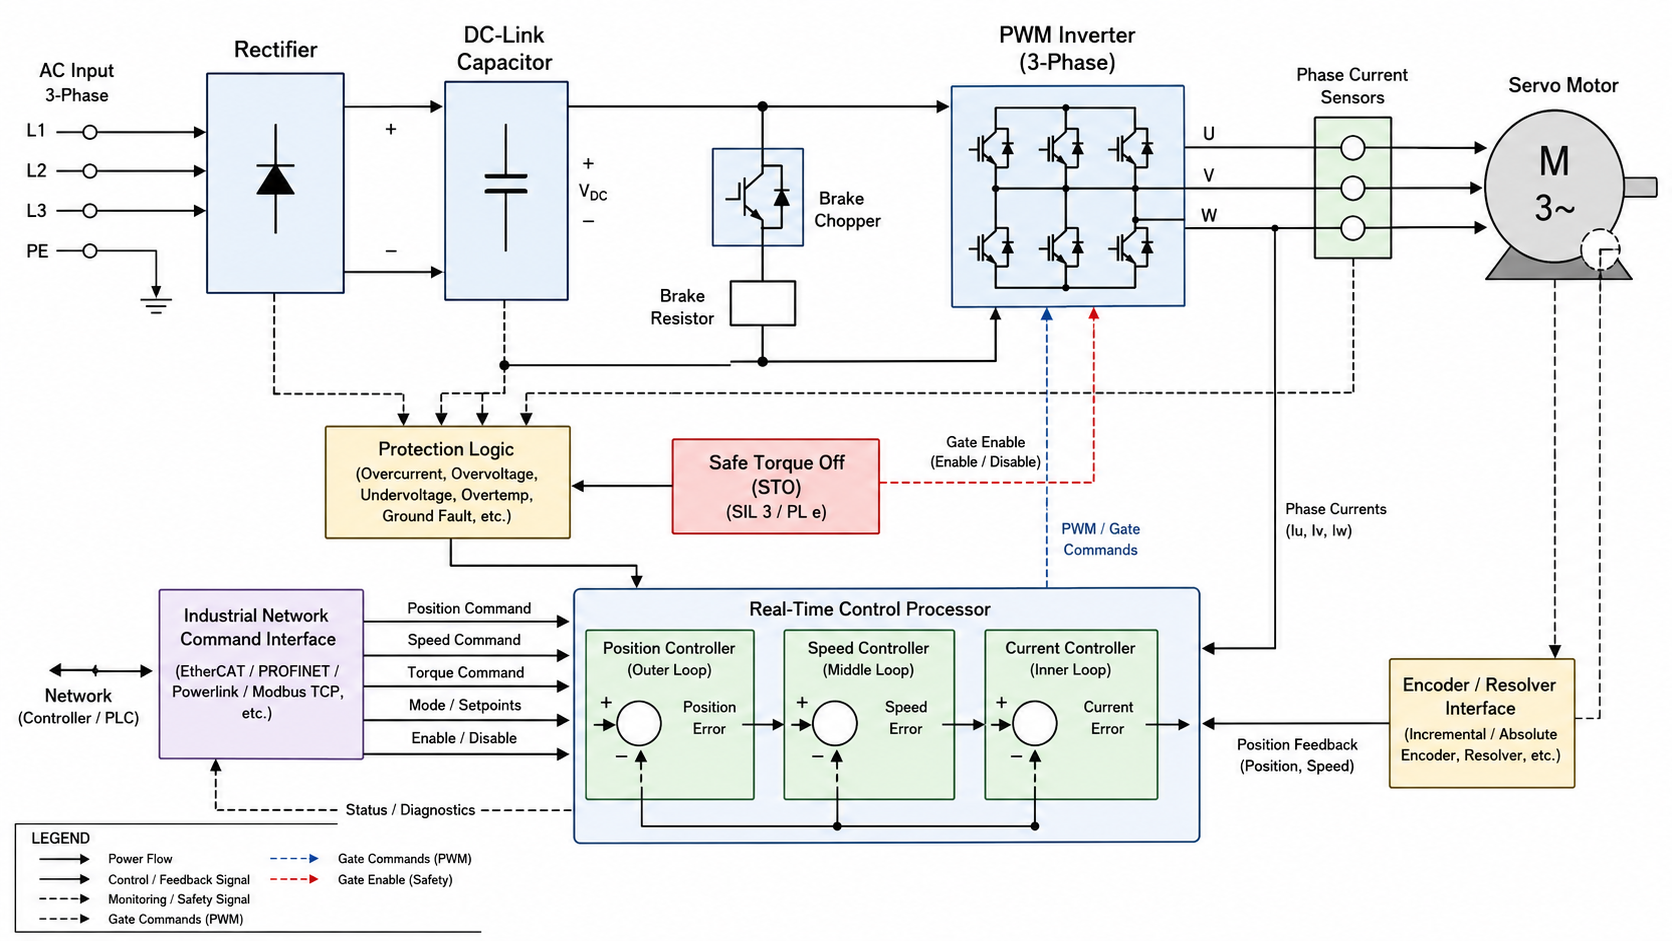
\includegraphics[width=0.8\textwidth]{images/chapter5/figure-9.png}
    \caption{โครงสร้างภายใน Servo Drive}
\end{figure}

\subsubsection{วงรอบควบคุมแบบซ้อน}

\paragraph{วงรอบกระแสหรือแรงบิด}

วงรอบกระแสเป็นชั้นในสุดและตอบสนองเร็วที่สุด ทำให้กระแสจริงติดตามกระแสอ้างอิง เนื่องจากแรงบิดมอเตอร์แปรผันกับกระแสโดยประมาณ

\[
T_m=K_t i_q
\]

สำหรับมอเตอร์แม่เหล็กถาวรที่ใช้ Field-Oriented Control กระแสแกน $q$ เป็นตัวสร้างแรงบิดหลักภายใต้เงื่อนไขทั่วไป วงรอบกระแสใช้เซนเซอร์กระแส ADC ตัวควบคุม PI และ PWM เพื่อสั่ง Inverter เอกสาร TI ระบุว่าวงรอบกระแสมีผลจำกัดสมรรถนะสูงสุดของวงรอบความเร็วและตำแหน่ง [3]

\[
u_i(t)=K_{pi}e_i(t)+K_{ii}\int e_i(t)\,dt
\]

\paragraph{วงรอบความเร็ว}

\[
e_\omega(t)=\omega^\ast(t)-\omega(t)
\]

\[
T^\ast(t)=K_{p\omega}e_\omega(t)
+K_{i\omega}\int e_\omega(t)\,dt
\]

พจน์อินทิกรัลช่วยลดความคลาดเคลื่อนคงค้างเมื่อมีแรงบิดโหลด แต่ Gain สูงเกินไปอาจเกิดการสั่น Overshoot และเสียงจากกลไก

\paragraph{วงรอบตำแหน่ง}

\[
e_\theta(t)=\theta^\ast(t)-\theta(t)
\]

ตัวควบคุมพื้นฐานอาจเป็นสัดส่วน

\[
\omega^\ast(t)=K_{p\theta}e_\theta(t)
\]

ระบบจริงอาจเพิ่ม Feedforward

\[
\omega^\ast
=
K_{p\theta}e_\theta
+
K_{vff}\dot{\theta}^\ast
+
K_{aff}\ddot{\theta}^\ast
\]

Feedforward ช่วยลด Following Error แต่ไม่ควรใช้แทนการทำให้ Feedback Loop เสถียร

\paragraph{ลำดับความเร็วของวงรอบ}

\[
\text{Current Loop}
>
\text{Velocity Loop}
>
\text{Position Loop}
\]

หมายถึงแบนด์วิดท์และอัตราการอัปเดตของวงรอบชั้นในต้องสูงกว่าชั้นนอกอย่างเพียงพอ ไม่ได้หมายความว่า Gain ตัวเลขของวงรอบกระแสต้องสูงกว่าเสมอ เพราะหน่วยและสเกลต่างกัน

% [รูปที่ 10: วงรอบกระแส ความเร็ว และตำแหน่งแบบซ้อน]
% ประเภทภาพ: Block Diagram
% ตำแหน่งที่แนะนำ: หลังหัวข้อ 7.11.4
% วัตถุประสงค์การเรียนรู้: อธิบายลำดับการสร้างคำสั่งและสัญญาณป้อนกลับ
% คำอธิบายภาพ: Position Command เข้าวงรอบ Position Controller สร้าง Speed Command; Speed Controller สร้าง Torque/Current Command; Current Controller สร้าง PWM ไปยัง Inverter และ Motor; Encoder ให้ Position/Velocity Feedback; Current Sensor ให้ Current Feedback
% องค์ประกอบที่ต้องมี: Position loop, velocity loop, current loop, inverter, motor, encoder, current sensor
% ข้อความหรือป้ายกำกับ: Outer Loop, Middle Loop, Inner Loop, Fastest Loop
% ภาษาของป้ายกำกับ: อังกฤษ
% สัดส่วนภาพ: 16:9
% Image Generation Prompt: Academic nested servo control-loop block diagram. Position command enters outer position controller and produces speed command. Middle speed controller produces torque/current command. Inner current controller drives PWM inverter and servo motor. Encoder provides position and derived velocity feedback; current sensors provide current feedback. Clearly show loop nesting and label current loop as fastest. Clean white background, blue technical textbook style, 16:9.
% Alt Text: แผนภาพวงรอบตำแหน่ง ความเร็ว และกระแสซ้อนกันในระบบเซอร์โว

\begin{figure}[htbp]
    \centering
    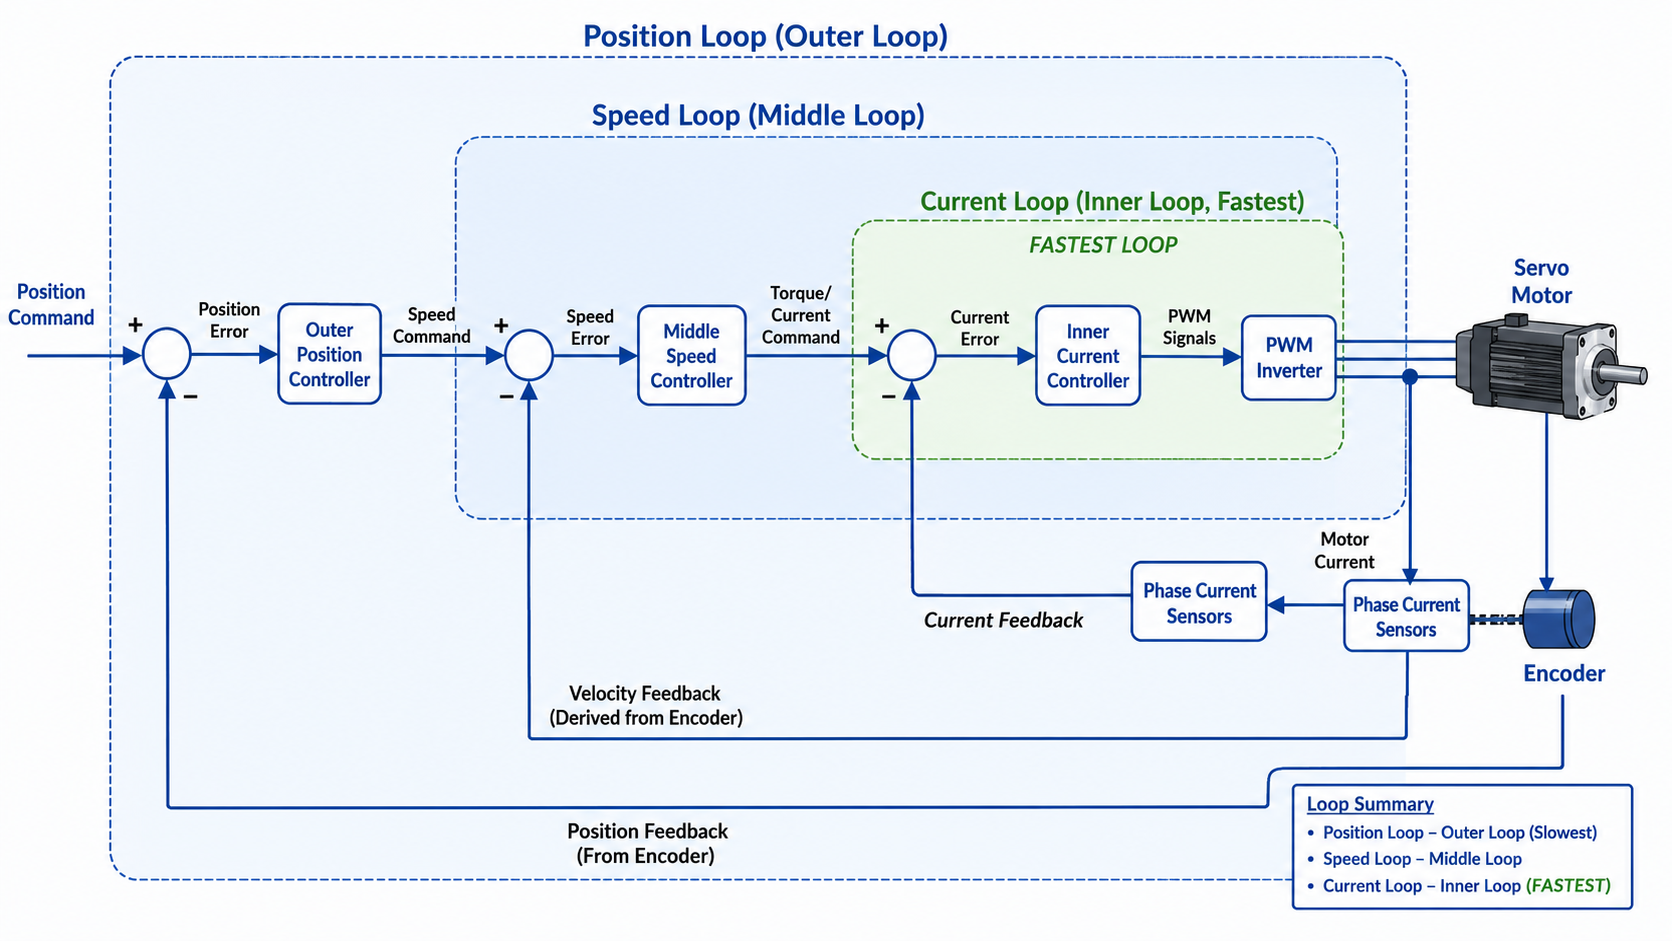
\includegraphics[width=0.8\textwidth]{images/chapter5/figure-10.png}
    \caption{วงรอบกระแส ความเร็ว และตำแหน่งแบบซ้อน}
\end{figure}

\subsubsection{การควบคุมแรงบิด ความเร็ว และตำแหน่ง}

\paragraph{Torque Control Mode}

Drive รับคำสั่งแรงบิดหรือกระแสโดยตรง เหมาะกับงานควบคุมแรงกด การขัน การพันวัสดุ หรือระบบที่ Controller ภายนอกปิดวงรอบเอง หากไม่มีวงรอบความเร็วภายนอก มอเตอร์อาจเร่งเมื่อโหลดต่ำ จึงต้องตั้ง Speed Limit

\paragraph{Velocity Control Mode}

Drive รับคำสั่งความเร็วและปิดวงรอบความเร็วภายใน เหมาะกับสายพาน ลูกกลิ้ง หรือ Spindle ต้องตั้ง Acceleration/Deceleration Limit เพื่อป้องกันกระแสสูงและแรงกระชาก

\paragraph{Position Control Mode}

Drive รับคำสั่งตำแหน่งผ่านพัลส์หรือเครือข่าย เหมาะกับแกนหยิบวาง โต๊ะ XY หรือกลไกที่ต้องหยุดตามพิกัด ควรตรวจ Electronic Gear, หน่วยตำแหน่ง, Homing, Limit และ Following Error Limit

\paragraph{ความสัมพันธ์ระหว่างโหมด}

เมื่อทำ Position Control ภายใน Drive มักยังใช้ Velocity Loop และ Current Loop อยู่ภายใน เพียงแต่ผู้ใช้ส่งคำสั่งที่ระดับตำแหน่ง ส่วน Torque Mode เปิดให้ Controller ภายนอกกำหนดคำสั่งชั้นในมากขึ้น

\subsubsection{ชุดเกียร์ อัตราทด และโมเมนต์ความเฉื่อยสะท้อน}

กำหนดอัตราทด

\[
n=\frac{\omega_m}{\omega_L}
\]

เมื่อพิจารณาประสิทธิภาพ $\eta_g$

\[
T_L=\eta_g n T_m
\]

ดังนั้น

\[
T_m=\frac{T_L}{\eta_g n}
\]

โมเมนต์ความเฉื่อยสะท้อน

\[
J_{\text{ref}}=\frac{J_L}{n^2}
\]

โมเมนต์ความเฉื่อยรวม

\[
J_{\text{total}}=J_m+J_{\text{gear}}+J_{\text{ref}}
\]

แรงบิดเร่ง

\[
T_{\text{acc}}=J_{\text{total}}\alpha
\]

แรงบิดรวมโดยประมาณ

\[
T_m=T_{\text{acc}}+T_{\text{load,ref}}+T_f
\]

การตรวจความร้อนใช้ RMS Torque

\[
T_{\text{RMS}}
=
\sqrt{
\frac{
T_1^2t_1+T_2^2t_2+\cdots+T_k^2t_k
}{
t_1+t_2+\cdots+t_k
}
}
\]

ต้องมี $T_{\text{RMS}}\leq T_{\text{continuous}}$ และแรงบิดสูงสุดต้องไม่เกิน Peak Torque ตามช่วงเวลาที่อนุญาต

% [รูปที่ 11: อัตราทดและโมเมนต์ความเฉื่อยสะท้อน]
% ประเภทภาพ: Technical Illustration
% ตำแหน่งที่แนะนำ: หลังหัวข้อ 7.13
% วัตถุประสงค์การเรียนรู้: แสดงผลของชุดเกียร์ต่อความเร็ว แรงบิด และโมเมนต์ความเฉื่อย
% คำอธิบายภาพ: มอเตอร์มี $J_m$, $\omega_m$, $T_m$ ต่อกับ Gear Ratio $n$ และ Efficiency $\eta_g$ ไปยังโหลด $J_L$, $\omega_L$, $T_L$ พร้อมสมการ $J_{\text{ref}}=J_L/n^2$
% องค์ประกอบที่ต้องมี: Motor, gearbox, load inertia, torque and speed arrows
% ข้อความหรือป้ายกำกับ: Reflected Inertia, Torque Multiplication, Speed Reduction
% ภาษาของป้ายกำกับ: อังกฤษ
% สัดส่วนภาพ: 16:9
% Image Generation Prompt: Engineering textbook illustration of a servo motor driving a robot joint through a gearbox. Label motor inertia Jm, motor speed omega_m, motor torque Tm, gear ratio n and efficiency eta_g, load inertia JL, load speed omega_L, and load torque TL. Include the equation J_ref = JL/n^2 and arrows showing speed reduction and torque multiplication. White background, 16:9.
% Alt Text: ภาพมอเตอร์ต่อชุดเกียร์และโหลด แสดงผลของอัตราทดต่อแรงบิด ความเร็ว และโมเมนต์ความเฉื่อยสะท้อน

\begin{figure}[htbp]
    \centering
    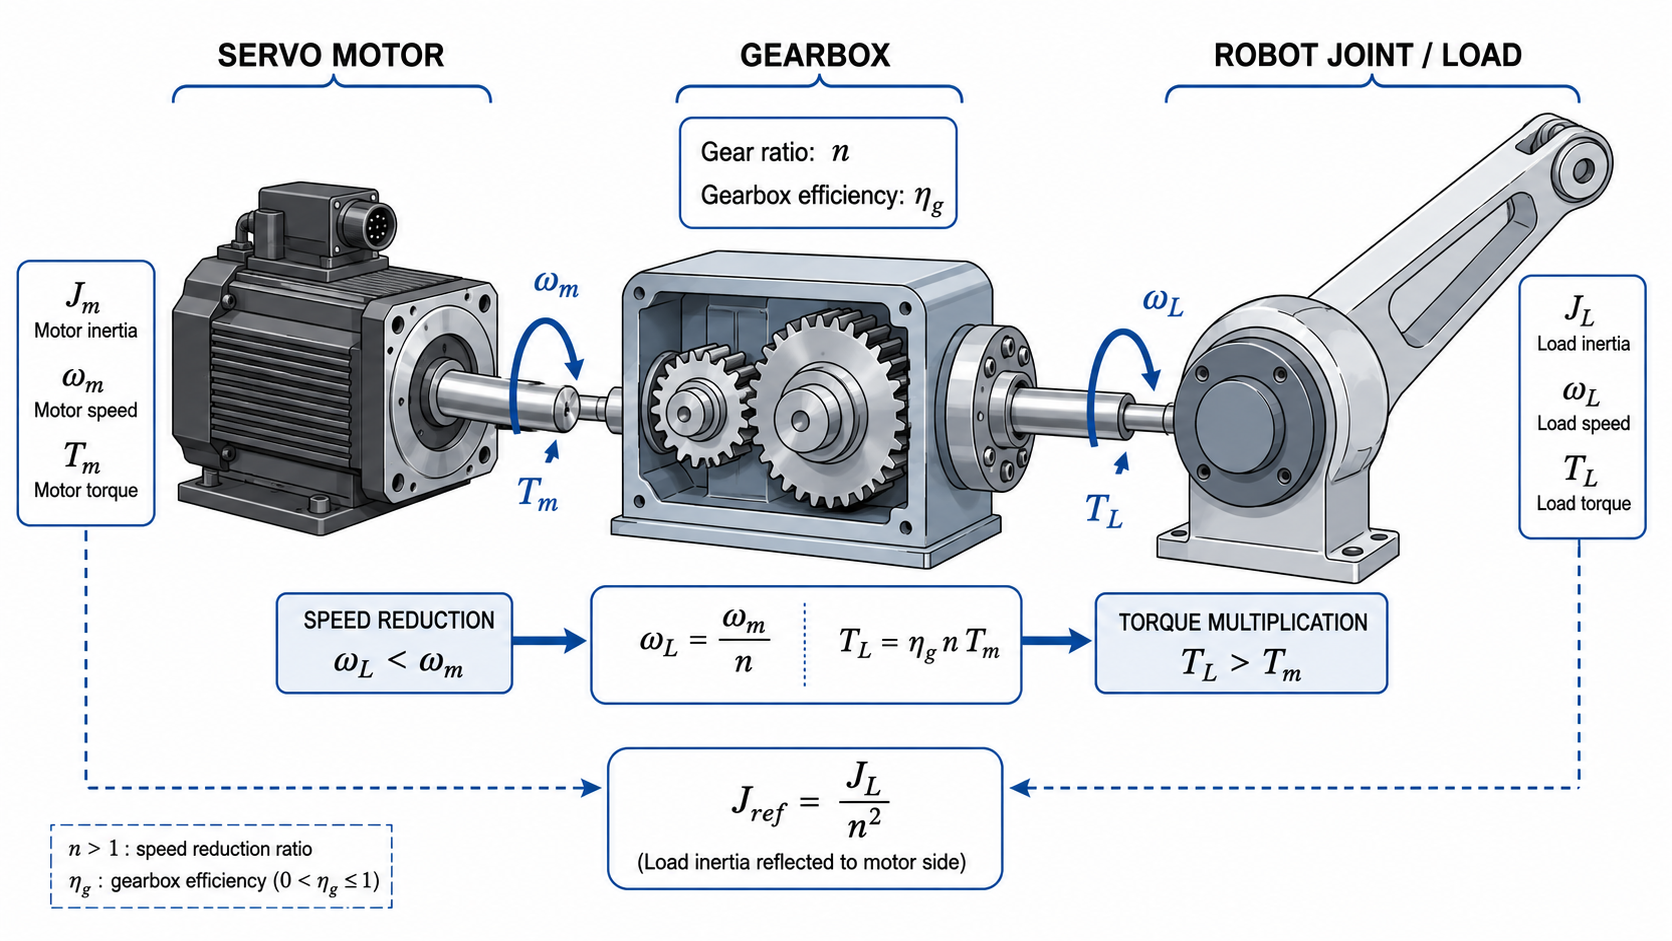
\includegraphics[width=0.8\textwidth]{images/chapter5/figure-11.png}
    \caption{อัตราทดและโมเมนต์ความเฉื่อยสะท้อน}
\end{figure}

\paragraph{ตัวอย่างที่ 7 ตัวอย่างเพิ่มเติมเพื่อการเรียนรู้: เลือกแรงบิดมอเตอร์เบื้องต้น}

แกนหนึ่งมี $J_{\text{total}}=0.0025\ \text{kg·m}^2$ ต้องเร่งจากหยุดนิ่งถึง $120\ \text{r/min}$ ใน $0.20\ \text{s}$ มีแรงบิดโหลดสะท้อน $1.20\ \text{N·m}$ และแรงเสียดทาน $0.10\ \text{N·m}$

\[
\omega_f=\frac{2\pi(120)}{60}=12.566\ \text{rad/s}
\]

\[
\alpha=\frac{12.566}{0.20}=62.83\ \text{rad/s}^2
\]

\[
T_{\text{acc}}=(0.0025)(62.83)=0.157\ \text{N·m}
\]

\[
T_m=0.157+1.20+0.10=1.457\ \text{N·m}
\]

ใช้ Safety Margin 1.5

\[
T_{\text{select}}=1.5(1.457)=2.19\ \text{N·m}
\]

ควรเลือกมอเตอร์ที่มี Peak Torque มากกว่า \textbf{2.19 N·m} และตรวจ RMS Torque, ความเร็วสูงสุด, Inertia Ratio และ Torque–Speed เพิ่มเติม

\subsubsection{การเลือกระบบขับเคลื่อนสำหรับแกนหุ่นยนต์}

\begin{enumerate}
    \item กำหนดภารกิจ ระยะ มุม ความเร็ว Cycle Time และ Repeatability
    \item กำหนดโหลด มวล จุดศูนย์ถ่วง Tool และแรงภายนอก
    \item สร้าง Motion Profile ช่วงเร่ง คงที่ ชะลอ และหยุด
    \item คำนวณแรงหรือแรงบิด
    \item เลือก Electric, Pneumatic หรือ Hydraulic
    \item กำหนดอัตราทดและกลไก
    \item ตรวจ Peak และ RMS Torque
    \item เลือก Feedback
    \item ตรวจพลังงาน Regeneration และความร้อน
    \item ตรวจความปลอดภัยและการบำรุงรักษา
    \item ตรวจความเข้ากันได้ Motor–Drive–Cable–Feedback–Controller
    \item ทดสอบและปรับจูนด้วยความเร็วต่ำก่อน
\end{enumerate}

\begin{table}[htbp]
    \centering
    \begin{tabular}{l l l}
        \hline
        \textbf{ความต้องการ} & \textbf{ทางเลือกเด่น} & \textbf{เหตุผล} \\
        \hline
        ตำแหน่งละเอียด วิถีต่อเนื่อง & AC Servo + Absolute Encoder & วงปิด ความละเอียดสูง และลด Homing \\
        ช่วงสั้น โหลดคงที่ ต้นทุนจำกัด & Stepper/Closed-Loop Stepper & ควบคุมด้วยพัลส์และติดตั้งง่าย \\
        Gripper เปิด–ปิด & Pneumatic Cylinder & โครงสร้างง่ายและตอบสนองเร็ว \\
        แรงสูงมาก พื้นที่ตัวกระทำจำกัด & Hydraulic Actuator & ความหนาแน่นกำลังสูง \\
        สภาพแวดล้อมสั่นและร้อน & Servo + Resolver & Feedback ทนทาน \\
        แกนแนวตั้ง & Servo + Holding Brake & ลดความเสี่ยงตกเมื่อปิดกำลัง \\
        \hline
    \end{tabular}
\end{table}

\subsubsection{การตั้งค่าและการปรับจูน Servo}

\paragraph{การตรวจสอบก่อนจ่ายกำลัง}

\begin{itemize}
    \item ตรวจรุ่น Motor และ Drive
    \item ตรวจแรงดันไฟเข้าและการต่อลงดิน
    \item ตรวจสาย Motor Power, Encoder และ Brake
    \item ตรวจ E-stop, Guard, Limit และ STO
    \item ยึดมอเตอร์และโหลดให้แน่น
    \item ตั้ง Current Limit, Speed Limit และ Travel Limit ต่ำในระยะแรก
    \item ตรวจทิศทางบวกและทิศทาง Feedback
    \item ห้ามบุคคลอยู่ในแนวการเคลื่อนที่
\end{itemize}

\paragraph{ลำดับการปรับจูน}

\begin{enumerate}
    \item ตั้งข้อมูลมอเตอร์และ Feedback
    \item Jog ที่ความเร็วต่ำ
    \item ตรวจทิศทาง
    \item ใช้ Auto-Tuning หากรองรับ
    \item ปรับ Velocity Gain ให้เร็วโดยไม่สั่น
    \item ปรับ Position Gain ให้ Following Error ต่ำ
    \item ใช้ Filter/Notch เมื่อระบุ Resonance ได้
    \item ทดสอบหลายตำแหน่งและโหลด
    \item ตรวจ Peak Current, RMS Torque, Temperature และ Alarm
    \item บันทึกพารามิเตอร์เวอร์ชันที่ผ่านการทดสอบ
\end{enumerate}

\begin{table}[htbp]
    \centering
    \begin{tabular}{l l l}
        \hline
        \textbf{อาการ} & \textbf{สาเหตุที่เป็นไปได้} & \textbf{แนวทางตรวจสอบ} \\
        \hline
        สั่นขณะหยุด & Position Gain สูง โครงสร้างยืดหยุ่น Feedback Noise & ลด Gain ตรวจคัปปลิงและสาย \\
        Overshoot สูง & Gain สูง Damping ต่ำ Feedforward มาก & ลด Gain/Feedforward \\
        Following Error สูง & Gain ต่ำ Torque Limit ต่ำ โหลดสูง & ตรวจ Current Limit และกลไก \\
        เสียงความถี่เฉพาะ & Mechanical Resonance & วัดความถี่ ใช้ Notch อย่างมีเหตุผล \\
        Overcurrent & ชน โหลดติด Acceleration สูง หรือสายผิด & ตัดกำลัง ตรวจสาเหตุ \\
        Overvoltage ตอนชะลอ & พลังงานคืนสูง Braking ไม่พอ & เพิ่มเวลาชะลอ ตรวจ Regeneration \\
        Encoder Alarm & สายขาด รบกวน หรือรุ่นไม่ตรง & ตรวจ Shield, Connector, Motor ID \\
        แกนตกเมื่อปิด Servo & Brake ไม่ทำงาน/ลำดับผิด & ตรวจ Holding Brake \\
        \hline
    \end{tabular}
\end{table}

\subsubsection{ความปลอดภัยของระบบขับเคลื่อน}

ระบบขับเคลื่อนมีพลังงานสะสมใน DC Bus มวลหมุน ลมอัด ของไหลแรงดัน สปริง และพลังงานศักย์ของแกนแนวตั้ง การกด E-stop ไม่ได้ทำให้พลังงานทุกชนิดหายไปทันที

\begin{enumerate}
    \item ปฏิบัติตาม ISO 10218-1:2025 และ ISO 10218-2:2025 [1], [2]
    \item ประเมินความเสี่ยงก่อนทดลอง
    \item แยก Emergency Stop, Protective Stop และ STO ตามหน้าที่
    \item รอเวลาคายประจุ DC Bus ตามคู่มือ
    \item ระบายและล็อกแรงดันลมหรือไฮดรอลิกก่อนซ่อม
    \item ใช้ Lockout/Tagout ตามระเบียบหน่วยงาน
    \item ห้ามใช้ Holding Brake แทนเบรกฉุกเฉิน
    \item ใช้ Guard, Interlock และ Safe Speed
    \item เดินสายกำลังและ Feedback แยกกัน
    \item บันทึก Fault และแก้สาเหตุก่อน Reset
\end{enumerate}

\par\noindent\rule{\textwidth}{0.4pt}\par

\subsection{ความเข้าใจผิดที่พบบ่อย}

\begin{enumerate}
    \item \textbf{Servo Motor คือมอเตอร์งานอดิเรกชนิดหนึ่ง} — ที่ถูกต้องคือ Servo เป็นระบบที่มีตัวกระทำ Feedback และวงรอบควบคุม
    \item \textbf{Servo Amplifier เพียงเพิ่มแรงดัน} — จริง ๆ ทำทั้งแปลงกำลัง ควบคุมวงรอบ อ่าน Feedback สื่อสาร และป้องกัน
    \item \textbf{Encoder Resolution สูงทำให้ปลายแขนแม่นยำเท่ากันเสมอ} — ยังขึ้นกับ Accuracy, Backlash, ความยืดหยุ่น และการสอบเทียบ
    \item \textbf{Stepper แบบวงเปิดไม่มีวันผิดตำแหน่ง} — อาจหลุดก้าวเมื่อโหลดหรือความเร่งสูง
    \item \textbf{Microstepping เพิ่ม Accuracy ตามจำนวน Microstep} — มักช่วยความเรียบมากกว่าความถูกต้องเชิงกลแบบสัดส่วนตรง
    \item \textbf{นิวเมติกให้แรงตาม @@LATEXTOKEN0@@ ทุกสถานการณ์} — แรงจริงต่ำลงจากแรงเสียดทานและความดันตก
    \item \textbf{เพิ่ม Gain มากทำให้ระบบดีขึ้นเสมอ} — อาจเกิด Oscillation, Noise และ Resonance
    \item \textbf{Holding Brake ใช้หยุดจากความเร็วสูงได้เป็นปกติ} — ส่วนมากใช้ยึดเมื่อหยุด ต้องตรวจคู่มือรุ่นจริง
\end{enumerate}

\par\noindent\rule{\textwidth}{0.4pt}\par

\subsection{การประยุกต์ใช้ในงานจริง}

\subsubsection{หุ่นยนต์เชื่อมอาร์ก}

ต้องการวิถีต่อเนื่อง ความเร็วสม่ำเสมอ และการประสานหลายแกน จึงนิยม AC Servo, Absolute Encoder และเครือข่าย Motion แบบเวลาจริง

\subsubsection{หุ่นยนต์หยิบวางความเร็วสูง}

ต้องการ Peak Torque สูงในช่วงเร่งและชะลอ การเลือกมอเตอร์ต้องตรวจ Peak และ RMS Torque รวมทั้งมวล Tool และชิ้นงาน

\subsubsection{Gripper แบบนิวเมติก}

เหมาะกับการเปิด–ปิดสองตำแหน่ง ควรใช้ Pressure Regulator, Flow Control และ Position Sensor หากชิ้นงานเปราะอาจใช้ Servo Gripper เพื่อควบคุมแรงละเอียดกว่า

\subsubsection{แกนแนวตั้ง}

ต้องคำนึงถึงแรงโน้มถ่วงตลอดเวลา ควรมี Holding Brake และลำดับปลดเบรกที่ถูกต้อง อาจใช้ Counterbalance เพื่อลดแรงบิดต่อเนื่อง

\subsubsection{หุ่นยนต์งานหนักแบบไฮดรอลิก}

เหมาะกับงานแรงสูง การควบคุมตำแหน่งละเอียดต้องใช้วาล์วสัดส่วน/Servo Valve ร่วมกับ Position และ Pressure Sensor พร้อม Relief Valve

\subsubsection{กรณีศึกษา: สถานีหยิบกล่อง}

ต้องหยิบกล่อง 5 kg ระยะ 0.6 m ความสามารถทำซ้ำ $\pm0.2$ mm Cycle Time 4 s และเปลี่ยนหลายตำแหน่ง จึงควรใช้ Servo มากกว่ากระบอกลมแบบสองตำแหน่ง ควรพิจารณา Absolute Encoder, ชุดเกียร์ Backlash ต่ำ, Peak/RMS Torque, Holding Brake สำหรับแกนแนวตั้ง และ Guard/Interlock

\par\noindent\rule{\textwidth}{0.4pt}\par

\subsection{สรุปท้ายบท}

\begin{enumerate}
    \item ระบบขับเคลื่อนประกอบด้วยแหล่งพลังงาน ตัวแปลงกำลัง ตัวกระทำ ชุดส่งกำลัง ตัวตรวจจับ ตัวควบคุม และความปลอดภัย
    \item ระบบไฟฟ้าเหมาะกับการควบคุมละเอียด นิวเมติกเหมาะกับงานเปิด–ปิด ไฮดรอลิกเหมาะกับงานแรงสูง
    \item มอเตอร์ DC มีความสัมพันธ์ $T=K_ti$ และ $e_b=K_e\omega$
    \item Stepper ควบคุมมุมจากพัลส์ แต่อาจหลุดก้าวเมื่อวงเปิด
    \item Servo Motor ทำงานร่วมกับ Drive และ Feedback
    \item Incremental Encoder ต้องอาศัยจุดอ้างอิง ส่วน Absolute Encoder รายงานตำแหน่งตามชนิด
    \item Resolver ทนสภาพแวดล้อมรุนแรงและใช้สัญญาณ Sine/Cosine
    \item วงรอบเซอร์โวเรียง Current/Torque, Velocity และ Position
    \item ชุดเกียร์เพิ่มแรงบิด ลดความเร็ว และลดความเฉื่อยสะท้อนตาม $J_{\text{ref}}=J_L/n^2$
    \item การเลือกมอเตอร์ต้องตรวจ Peak, RMS, Speed, Inertia, Feedback, Regeneration และ Compatibility
    \item การปรับจูนต้องเริ่มด้วยข้อจำกัดที่ปลอดภัยและวิเคราะห์ Resonance
    \item การทดลองต้องมี E-stop, Guard, STO และขั้นตอนตัดแยกพลังงาน
\end{enumerate}

\par\noindent\rule{\textwidth}{0.4pt}\par

\newpage

\subsection{คำถามทบทวน}

\begin{enumerate}
    \item Servo Motor, Servo Drive และ Servo Amplifier ต่างกันอย่างไร
    \item เพราะเหตุใดระบบไฟฟ้าจึงนิยมในหุ่นยนต์สมัยใหม่
    \item เปรียบเทียบนิวเมติกกับไฮดรอลิก
    \item อธิบายความหมายของ $T=K_ti$ และ $e_b=K_e\omega$
    \item เพราะเหตุใด Stepper แบบวงเปิดจึงสูญเสียตำแหน่งได้
    \item Resolution, Accuracy และ Repeatability ต่างกันอย่างไร
    \item Incremental และ Absolute Encoder มีผลต่อ Homing ต่างกันอย่างไร
    \item อธิบายหน้าที่ Current, Velocity และ Position Loop
    \item อัตราทดมีผลต่อแรงบิด ความเร็ว และความเฉื่อยอย่างไร
    \item Overvoltage ระหว่างชะลอเกิดจากอะไร
    \item เหตุใด Holding Brake ไม่ควรแทนเบรกฉุกเฉิน
    \item ระบุรายการตรวจสอบห้าข้อก่อน Enable Servo
\end{enumerate}

\subsection{กิจกรรมปฏิบัติการ}

\subsection{กิจกรรมปฏิบัติการที่ 1: เปรียบเทียบ Stepper แบบวงเปิดกับ Servo แบบวงปิด}

\subsubsection{วัตถุประสงค์}

\begin{enumerate}
    \item สั่งการเคลื่อนที่ของ Stepper และ Servo บนชุดฝึกแรงดันต่ำได้
    \item วัดตำแหน่งหรือจำนวนรอบภายใต้โหลดที่เปลี่ยนแปลงได้
    \item เปรียบเทียบการหลุดก้าว Following Error และการตอบสนองต่อโหลดได้
    \item ปฏิบัติงานตามขั้นตอนความปลอดภัยได้
\end{enumerate}

\subsubsection{หลักการและทฤษฎีที่เกี่ยวข้อง}

Stepper แบบวงเปิดเชื่อว่าตำแหน่งจริงติดตามจำนวนพัลส์คำสั่ง หากแรงบิดไม่เพียงพออาจหลุดก้าวโดย Controller ไม่ทราบ ส่วน Servo ใช้ Encoder ป้อนกลับและ Drive ปรับกระแสเพื่อลด Error

\subsubsection{อุปกรณ์ เครื่องมือ และซอฟต์แวร์}

\begin{itemize}
    \item ชุดฝึก Stepper Motor และ Driver ไม่เกิน 24 VDC
    \item ชุดฝึก Servo Motor และ Servo Drive สำหรับการศึกษา
    \item แหล่งจ่าย DC แบบจำกัดกระแส
    \item Encoder Counter หรือ Motion Controller ที่อ่าน Actual Position ได้
    \item โหลดปรับค่าได้ที่มีฝาครอบ
    \item Tachometer หรือ Oscilloscope ตามความเหมาะสม
    \item Emergency Stop และ Guard
    \item แบบบันทึกผล
\end{itemize}

\subsubsection{แผนภาพหรือวงจร}

% [รูปที่ 12: ชุดทดลองเปรียบเทียบ Stepper และ Servo]
% ประเภทภาพ: Experimental Setup
% ตำแหน่งที่แนะนำ: หัวข้อ 4 ของกิจกรรมปฏิบัติการที่ 1
% วัตถุประสงค์การเรียนรู้: แสดงการเชื่อมต่ออุปกรณ์อย่างปลอดภัยและจุดวัด
% คำอธิบายภาพ: ซ้ายเป็น 24 VDC Supply → Stepper Driver → Stepper Motor → Covered Load พร้อม Command Pulse Counter ขวาเป็น Prewired Servo Drive Trainer → Servo Motor → Covered Load พร้อม Encoder Feedback และหน้าจอ Command/Actual Position ทั้งสองชุดมี E-stop และ Guard
% องค์ประกอบที่ต้องมี: Low-voltage supply, drivers, motors, encoder, covered load, E-stop, guard, measurement points
% ข้อความหรือป้ายกำกับ: Command Position, Actual Position, Adjustable Load
% ภาษาของป้ายกำกับ: อังกฤษ
% สัดส่วนภาพ: 16:9
% Image Generation Prompt: Safe educational laboratory setup comparing an open-loop stepper axis and a closed-loop servo axis. Left: 24 VDC supply, stepper driver, stepper motor, pulse command counter, guarded adjustable load. Right: prewired educational servo drive, servo motor, encoder feedback, guarded adjustable load, display of command and actual position. Include emergency stop and protective guards. Clean technical illustration, white background, 16:9.
% Alt Text: ชุดฝึก Stepper และ Servo ที่มีโหลดปรับค่าได้ ฝาครอบ และอุปกรณ์หยุดฉุกเฉิน

\begin{figure}[htbp]
    \centering
    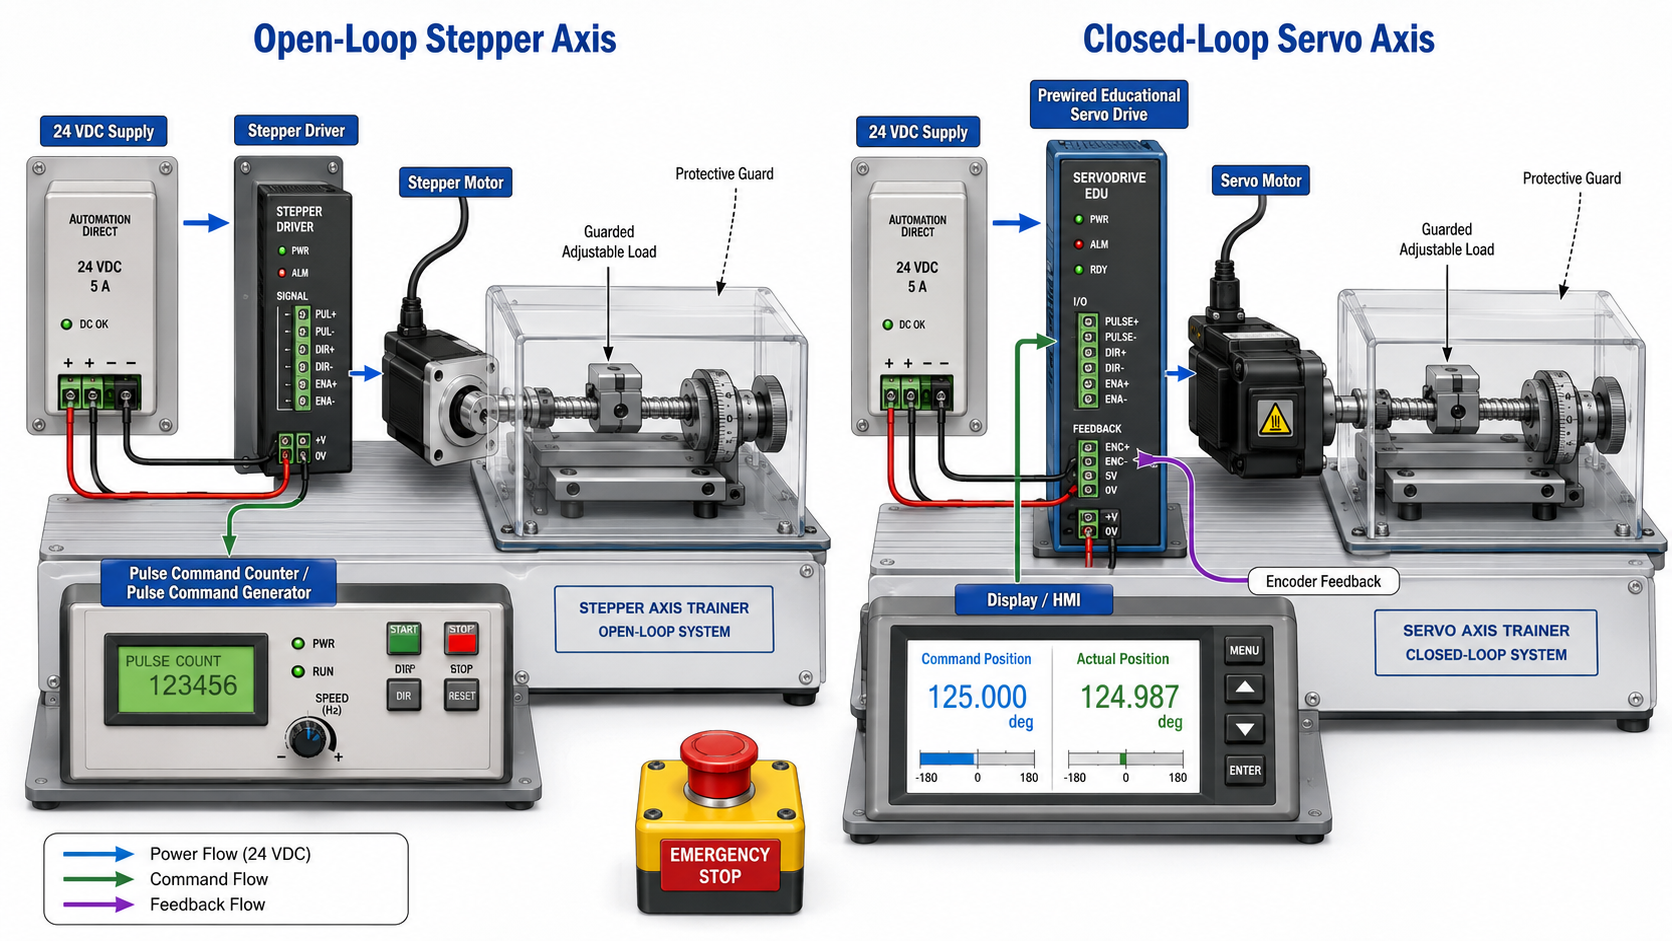
\includegraphics[width=0.8\textwidth]{images/chapter5/figure-12.png}
    \caption{ชุดทดลองเปรียบเทียบ Stepper และ Servo}
\end{figure}

\subsubsection{ข้อควรระวังด้านความปลอดภัย}

\begin{enumerate}
    \item ใช้เฉพาะชุดฝึกที่ผู้สอนเดินสายกำลังและตรวจสอบแล้ว
    \item ห้ามสัมผัสเพลา คัปปลิง หรือโหลดขณะ Enable
    \item ใช้ Guard ปิดชิ้นส่วนหมุนตลอดการทดลอง
    \item ตั้ง Speed Limit และ Current Limit ต่ำก่อนเริ่ม
    \item ปรับโหลดเมื่อระบบหยุดและตัด Enable แล้วเท่านั้น
    \item ทดสอบ E-stop ก่อนเริ่มทุกกลุ่ม
    \item ห้าม Reset Fault ซ้ำจนกว่าจะระบุสาเหตุได้
\end{enumerate}

\subsubsection{ขั้นตอนการปฏิบัติ}

\begin{enumerate}
    \item ตรวจสอบอุปกรณ์และ Guard
    \item บันทึกมุมก้าว Microstep Encoder Resolution และค่าจำกัดกระแส
    \item สั่ง Stepper เคลื่อนที่ 10 รอบที่ความเร็วต่ำโดยไม่มีโหลดเพิ่ม
    \item บันทึก Command Pulse และตำแหน่งจริง
    \item เพิ่มโหลดทีละระดับภายใต้การกำกับของผู้สอน
    \item ทำซ้ำที่ความเร่งสองระดับและบันทึกการหลุดก้าว
    \item ทดสอบ Servo ด้วย Motion Profile เดียวกัน
    \item บันทึก Command Position, Actual Position, Peak Following Error และ Peak Current
    \item เปรียบเทียบผล
    \item ลดความเร็ว ปิด Enable และตัดแหล่งจ่าย
\end{enumerate}

\subsubsection{ตารางบันทึกผล}

\begin{table}[htbp]
    \centering
    \begin{tabular}{l r r r r r r r l}
        \hline
        \textbf{ระบบ} & \textbf{โหลดระดับ} & \textbf{ความเร็ว} & \textbf{ความเร่ง} & \textbf{ตำแหน่งสั่ง} & \textbf{ตำแหน่งจริง} & \textbf{Error} & \textbf{Peak Current} & \textbf{ข้อสังเกต} \\
        \hline
        Stepper & 0 &  &  &  &  &  &  &  \\
        Stepper & 1 &  &  &  &  &  &  &  \\
        Stepper & 2 &  &  &  &  &  &  &  \\
        Servo & 0 &  &  &  &  &  &  &  \\
        Servo & 1 &  &  &  &  &  &  &  \\
        Servo & 2 &  &  &  &  &  &  &  \\
        \hline
    \end{tabular}
\end{table}

\subsubsection{การคำนวณและวิเคราะห์ผล}

\[
e_\theta=\theta_{\text{cmd}}-\theta_{\text{actual}}
\]

\[
\%\text{Error}
=
\frac{|e_\theta|}{|\theta_{\text{cmd}}|}\times100
\]

วิเคราะห์ความสัมพันธ์ระหว่างโหลด ความเร่ง กระแส และ Error โดยไม่แต่งค่าที่ไม่ได้วัด

\subsubsection{การเปรียบเทียบผลจริงกับทฤษฎี}

Stepper ควรติดตามพัลส์เมื่อแรงบิดสำรองเพียงพอ แต่จะหลุดก้าวเมื่อโหลดหรือความเร่งเกินขีดจำกัด Servo จะเพิ่มกระแสเพื่อต้านโหลดและลด Following Error จนถึง Torque Limit

\subsubsection{คำถามหลังการทดลอง}

\begin{enumerate}
    \item เงื่อนไขใดทำให้ Stepper เริ่มหลุดก้าว
    \item Servo Current เปลี่ยนอย่างไรเมื่อเพิ่มโหลด
    \item เหตุใด Servo ยังมี Following Error
    \item หากเพิ่ม Position Gain สูงเกินไปจะเกิดผลใด
    \item งานประเภทใดควรเลือก Stepper หรือ Servo
\end{enumerate}

\subsubsection{เกณฑ์การประเมิน}

\begin{table}[htbp]
    \centering
    \begin{tabular}{l r}
        \hline
        \textbf{เกณฑ์} & \textbf{คะแนน} \\
        \hline
        ความปลอดภัยและการตรวจสอบก่อนเริ่ม & 20 \\
        การตั้งค่าและใช้อุปกรณ์ถูกต้อง & 20 \\
        การบันทึกผลครบถ้วน & 20 \\
        การคำนวณและกราฟเปรียบเทียบ & 20 \\
        การอภิปรายผลและตอบคำถาม & 20 \\
        \textbf{รวม} & \textbf{100} \\
        \hline
    \end{tabular}
\end{table}

\par\noindent\rule{\textwidth}{0.4pt}\par

\subsection{กิจกรรมปฏิบัติการที่ 2: วัดความละเอียด ตำแหน่ง และความเร็วจาก Encoder}

\subsubsection{วัตถุประสงค์}

\begin{enumerate}
    \item อ่านสัญญาณ A, B และ Z ของ Incremental Encoder ได้
    \item คำนวณตำแหน่งและความเร็วจาก Count ได้
    \item ระบุทิศทางจากลำดับเฟส A/B ได้
    \item วิเคราะห์ผลของ Sampling Time ต่อความละเอียดการวัดความเร็วได้
\end{enumerate}

\subsubsection{หลักการและทฤษฎีที่เกี่ยวข้อง}

\[
\theta=\frac{360^\circ N_c}{C}
\]

\[
\omega \approx \frac{2\pi\Delta N_c}{C\Delta t}
\]

ช่วงเวลา $\Delta t$ สั้นตอบสนองเร็วแต่ Count น้อยและ Noise เชิงควอนไทซ์สูง ช่วงเวลายาวให้ค่าความเร็วเรียบขึ้นแต่ตอบสนองช้าลง

\subsubsection{อุปกรณ์ เครื่องมือ และซอฟต์แวร์}

\begin{itemize}
    \item มอเตอร์ DC หรือ Servo Trainer แรงดันต่ำ
    \item Incremental Encoder ที่ทราบ PPR/CPR
    \item Oscilloscope หรือ Logic Analyzer
    \item Counter/Timer หรือ Motion Controller
    \item แหล่งจ่ายที่จำกัดกระแส
    \item Guard และ E-stop
    \item Differential Input ตามชนิดสัญญาณ หากจำเป็น
\end{itemize}

\subsubsection{แผนภาพหรือวงจร}

ใช้แนวคิดจากรูปที่ 8 และเพิ่มจุดวัด A, B, Z และ Reference ตามคู่มือ Encoder

\subsubsection{ข้อควรระวังด้านความปลอดภัย}

\begin{itemize}
    \item ตรวจระดับแรงดัน Encoder ก่อนเชื่อมเครื่องมือวัด
    \item ห้ามต่อ Ground ของ Oscilloscope โดยไม่ตรวจศักย์อ้างอิง
    \item ห้ามจับเพลาหมุน
    \item ใช้ Differential Input เมื่อเป็น Line Driver
\end{itemize}

\subsubsection{ขั้นตอนการปฏิบัติ}

\begin{enumerate}
    \item บันทึก PPR และรูปแบบเอาต์พุต
    \item หมุนเพลาช้า ๆ และสังเกต A/B/Z
    \item บันทึกลำดับเฟสทั้งสองทิศ
    \item หมุนหนึ่งรอบและนับ Count
    \item เปรียบเทียบกับ $C=4PPR$ หากใช้ Quadrature x4
    \item สั่งความเร็วคงที่สามระดับ
    \item คำนวณความเร็วด้วย $\Delta t$ อย่างน้อยสามค่า
    \item เปรียบเทียบกับ Tachometer หรือค่าจาก Drive
    \item วิเคราะห์ Noise, Quantization และ Delay
\end{enumerate}

\subsubsection{ตารางบันทึกผล}

\begin{table}[htbp]
    \centering
    \begin{tabular}{r r r r r r}
        \hline
        \textbf{ความเร็วอ้างอิง} & \textbf{$\Delta t$} & \textbf{$\Delta N_c$} & \textbf{ความเร็วคำนวณ} & \textbf{ความเร็วจากเครื่องมือ} & \textbf{ความคลาดเคลื่อน} \\
        \hline
         &  &  &  &  &  \\
         &  &  &  &  &  \\
         &  &  &  &  &  \\
        \hline
    \end{tabular}
\end{table}

\subsubsection{การคำนวณและวิเคราะห์ผล}

\[
N=\frac{60\omega}{2\pi}
\]

\[
\%\text{Error}
=
\frac{|N_{\text{calc}}-N_{\text{ref}}|}{N_{\text{ref}}}\times100
\]

\subsubsection{การเปรียบเทียบผลจริงกับทฤษฎี}

พิจารณานิยาม PPR/CPR การนับขอบ สัญญาณรบกวน และการตั้งค่า Counter หาก Count ต่อรอบไม่ตรงกับที่คาด

\subsubsection{คำถามหลังการทดลอง}

\begin{enumerate}
    \item เหตุใด A และ B ต้องต่างเฟส
    \item ช่อง Z ใช้ประโยชน์อย่างไร
    \item Sampling Time มีผลต่อ Noise และ Delay อย่างไร
    \item ความละเอียดสูงช่วยการวัดความเร็วต่ำอย่างไร
    \item เหตุใดสาย Encoder ควรแยกจากสายมอเตอร์
\end{enumerate}

\subsubsection{เกณฑ์การประเมิน}

ใช้เกณฑ์เดียวกับกิจกรรมที่ 1 โดยเปลี่ยนหัวข้อการตั้งค่าเป็นความถูกต้องของการวัดสัญญาณและการคำนวณ

\par\noindent\rule{\textwidth}{0.4pt}\par

\subsection{กิจกรรมปฏิบัติการที่ 3: Commissioning และปรับจูน Servo Drive บนชุดฝึก}

\subsubsection{วัตถุประสงค์}

\begin{enumerate}
    \item ตรวจสอบรายการก่อน Enable Servo ได้
    \item ตั้ง Motor Data, Limit และ Homing Parameter ได้
    \item เปรียบเทียบการตอบสนองก่อนและหลัง Auto-Tuning ได้
    \item อ่านกราฟ Position, Speed, Current และ Following Error ได้
    \item ระบุอาการ Gain ต่ำ Gain สูง และ Resonance ได้อย่างปลอดภัย
\end{enumerate}

\subsubsection{หลักการและทฤษฎีที่เกี่ยวข้อง}

ใช้แนวคิดวงรอบซ้อน Position–Velocity–Current และ Motion Profile แบบ Trapezoidal หรือ S-Curve เป้าหมายการปรับจูนคือให้ระบบตอบสนองเร็วโดยไม่สั่นและไม่เกินขีดจำกัดกระแส

\subsubsection{อุปกรณ์ เครื่องมือ และซอฟต์แวร์}

\begin{itemize}
    \item Servo Trainer ที่ผู้สอนเดินสายกำลังสำเร็จ
    \item Motor และ Drive คู่รุ่นที่ผู้ผลิตรับรอง
    \item คอมพิวเตอร์และซอฟต์แวร์ตั้งค่าของผู้ผลิต
    \item โหลดเฉื่อยที่มี Guard
    \item E-stop, STO และ Limit Switch
    \item เครื่องมือบันทึกของ Drive
\end{itemize}

\subsubsection{แผนภาพหรือวงจร}

ใช้รูปที่ 9 และ 10 โดยระบุจุดบันทึก Position Command, Actual Position, Speed, Torque/Current และ Alarm

\subsubsection{ข้อควรระวังด้านความปลอดภัย}

\begin{enumerate}
    \item นักศึกษาไม่เปิดฝาครอบหรือแตะขั้วไฟกำลัง
    \item ผู้สอนเป็นผู้จ่ายไฟหลักและยืนยันเวลาคายประจุ
    \item ตั้งความเร็วไม่เกินค่าของชุดฝึก
    \item ใช้ Guard ตลอดเวลา
    \item ทดสอบ STO และ E-stop
    \item ห้ามปิดฟังก์ชันป้องกันเพื่อให้ทดลองผ่าน
    \item หากมีเสียงผิดปกติให้ Stop และตัด Enable
\end{enumerate}

\subsubsection{ขั้นตอนการปฏิบัติ}

\begin{enumerate}
    \item ตรวจ Model Motor/Drive/Cable
    \item อ่านและบันทึกพารามิเตอร์เดิม
    \item ตั้ง Current, Speed และ Travel Limit
    \item Jog ที่ความเร็วต่ำและตรวจทิศทาง
    \item สั่ง Position Step ขนาดเล็กและบันทึกกราฟ
    \item รัน Auto-Tuning ตามคู่มือ
    \item ทำ Motion Profile เดิมซ้ำ
    \item เปรียบเทียบ Rise Time, Overshoot, Settling Time, Peak Current และ Following Error
    \item ปรับ Position Gain ทีละขั้นในขอบเขตที่ผู้สอนกำหนด
    \item คืนค่าพารามิเตอร์ที่ผ่านการตรวจสอบ
\end{enumerate}

\subsubsection{ตารางบันทึกผล}

\begin{table}[htbp]
    \centering
    \begin{tabular}{l r r r r r l}
        \hline
        \textbf{ชุดพารามิเตอร์} & \textbf{Rise Time} & \textbf{Overshoot} & \textbf{Settling Time} & \textbf{Peak Following Error} & \textbf{Peak Current} & \textbf{การสั่น/เสียง} \\
        \hline
        ก่อน Tuning &  &  &  &  &  &  \\
        Auto-Tuning &  &  &  &  &  &  \\
        ปรับเพิ่มเติม &  &  &  &  &  &  \\
        \hline
    \end{tabular}
\end{table}

\subsubsection{การคำนวณและวิเคราะห์ผล}

\[
\%OS=\frac{y_{\max}-y_{\text{final}}}{y_{\text{final}}}\times100
\]

เปรียบเทียบ Following Error และ Settling Time โดยพิจารณา Peak Current และการสั่นร่วมด้วย

\subsubsection{การเปรียบเทียบผลจริงกับทฤษฎี}

อภิปรายว่าการเพิ่ม Gain ลด Error แต่เพิ่มความไวต่อ Resonance และ Noise อย่างไร รวมทั้งผลของ Load Inertia ต่อ Auto-Tuning

\subsubsection{คำถามหลังการทดลอง}

\begin{enumerate}
    \item ทำไมต้องจำกัด Speed และ Current ก่อน Jog
    \item Auto-Tuning ใช้แทนการตรวจกลไกได้หรือไม่
    \item กราฟใดช่วยแยกปัญหาโหลดติดกับ Gain ต่ำ
    \item Resonance แตกต่างจาก Overshoot ปกติอย่างไร
    \item เหตุใดต้องบันทึกพารามิเตอร์เวอร์ชันที่ผ่านการทดสอบ
\end{enumerate}

\subsubsection{เกณฑ์การประเมิน}

\begin{table}[htbp]
    \centering
    \begin{tabular}{l r}
        \hline
        \textbf{เกณฑ์} & \textbf{คะแนน} \\
        \hline
        ตรวจความปลอดภัยและ Checklist & 25 \\
        ตั้งค่าและทำตามลำดับ & 20 \\
        บันทึกกราฟและพารามิเตอร์ & 20 \\
        วิเคราะห์ผลการปรับจูน & 25 \\
        การทำงานเป็นทีมและรายงาน & 10 \\
        \textbf{รวม} & \textbf{100} \\
        \hline
    \end{tabular}
\end{table}

\subsection{แบบฝึกหัดท้ายบท}

\subsubsection{ระดับพื้นฐาน}

\begin{enumerate}
    \item จงอธิบายหน้าที่ของ Servo Drive อย่างน้อยห้าประการ
    \item มอเตอร์ DC มี $K_t=0.22\ \text{N·m/A}$ และกระแส 4 A จงหาแรงบิดแม่เหล็กไฟฟ้า
    \item Stepper Motor มีมุมก้าว $1.8^\circ$ จงหาจำนวน Full Step ต่อรอบ
    \item Absolute Encoder 18 บิตมีจำนวนตำแหน่งต่อรอบเท่าใด และมีความละเอียดเชิงมุมกี่องศาต่อ Count
    \item กระบอกลมเส้นผ่านศูนย์กลาง 25 mm ใช้ความดัน 5 bar จงหาแรงยืดทฤษฎี
\end{enumerate}

\subsubsection{ระดับวิเคราะห์}

\begin{enumerate}
    \setcounter{enumi}{5}
    \item Stepper $1.8^\circ$ ใช้ Microstepping 8 และชุดเกียร์ $n=10$ ต้องการให้โหลดหมุน $45^\circ$ ต้องใช้กี่พัลส์
    \item Incremental Encoder 2,500 PPR ใช้ Quadrature x4 หากนับได้ 12,500 Count ในเวลา 0.25 s จงหาความเร็วรอบต่อนาที
    \item Servo Motor ขับโหลดผ่านชุดเกียร์ $n=20$ ประสิทธิภาพ 0.90 โหลดต้องการแรงบิด 80 N·m จงหาแรงบิดมอเตอร์ขั้นต่ำเมื่อไม่คิดแรงเร่ง
    \item โหลดมีโมเมนต์ความเฉื่อย $J_L=0.80\ \text{kg·m}^2$ ต่อผ่านชุดเกียร์ $n=25$ จงหาโมเมนต์ความเฉื่อยสะท้อนที่เพลามอเตอร์
    \item ระบบมีแรงบิด 3 N·m เป็นเวลา 0.4 s, 1 N·m เป็นเวลา 1.2 s และ 0 N·m เป็นเวลา 0.4 s จงหา RMS Torque
\end{enumerate}

\subsubsection{ระดับประยุกต์ใช้}

\begin{enumerate}
    \setcounter{enumi}{10}
    \item สถานีหนึ่งต้องเปิด–ปิด Gripper สองตำแหน่ง ระยะ 30 mm เวลา 0.25 s แรงหนีบประมาณ 150 N และไม่ต้องควบคุมตำแหน่งกึ่งกลาง จงเลือกระบบ Electric Servo, Pneumatic หรือ Hydraulic พร้อมเหตุผลและอุปกรณ์ควบคุมที่จำเป็น
    \item แกนแนวตั้งต้องยกโหลดด้วยแรงบิดโหลดสะท้อน 1.8 N·m มีโมเมนต์ความเฉื่อยรวม $0.003\ \text{kg·m}^2$ และต้องเร่งถึง 200 r/min ใน 0.15 s แรงเสียดทาน 0.15 N·m จงคำนวณ Peak Torque และเสนอพิกัดมอเตอร์เบื้องต้นเมื่อใช้ Safety Margin 1.4
    \item ชุด Servo หลังเพิ่ม Position Gain มี Following Error ลดลง แต่เกิดเสียงสั่นที่ความถี่คงที่และ Peak Current สูงขึ้น จงวิเคราะห์สาเหตุ ลำดับตรวจสอบ และแนวทางแก้ไขที่ไม่ลดความปลอดภัย
\end{enumerate}

\par\noindent\rule{\textwidth}{0.4pt}\par

\subsection{แนวคำตอบและเฉลยสำหรับผู้สอน}

\subsubsection{เฉลยข้อ 1}

Servo Drive ทำหน้าที่รับคำสั่ง ควบคุมภาคกำลัง อ่าน Feedback ปิดวงรอบกระแส/ความเร็ว/ตำแหน่ง จำกัดกระแสและความเร็ว ตรวจ Fault จัดการ Regeneration สื่อสารกับ Controller และรองรับฟังก์ชันความปลอดภัยตามรุ่น

\subsubsection{เฉลยข้อ 2}

\[
T=K_ti=(0.22)(4)=0.88\ \text{N·m}
\]

ตอบ \textbf{0.88 N·m}

\subsubsection{เฉลยข้อ 3}

\[
N_s=\frac{360}{1.8}=200
\]

ตอบ \textbf{200 Full Step ต่อรอบ}

\subsubsection{เฉลยข้อ 4}

\[
C=2^{18}=262\,144
\]

\[
\Delta\theta=\frac{360}{262\,144}=0.001373^\circ
\]

ตอบ \textbf{262,144 ตำแหน่งต่อรอบ} และประมาณ \textbf{0.00137°/Count}

\subsubsection{เฉลยข้อ 5}

\[
D=0.025\ \text{m},\quad p=5\times10^5\ \text{Pa}
\]

\[
A=\frac{\pi(0.025)^2}{4}=4.909\times10^{-4}\ \text{m}^2
\]

\[
F=pA=(5\times10^5)(4.909\times10^{-4})=245.4\ \text{N}
\]

ตอบแรงทฤษฎีประมาณ \textbf{245 N} แรงจริงต่ำกว่าจากแรงเสียดทานและความดันตกคร่อม

\subsubsection{เฉลยข้อ 6}

\[
N_s=200,\qquad N_p=200(8)=1600
\]

\[
N_{\text{cmd}}
=
\frac{45}{360}(1600)(10)
=2000
\]

ตอบ \textbf{2,000 พัลส์}

\subsubsection{เฉลยข้อ 7}

\[
C=4(2500)=10\,000
\]

\[
n_r=\frac{12\,500}{10\,000}=1.25\ \text{rev}
\]

\[
N=\frac{1.25}{0.25}(60)=300\ \text{r/min}
\]

ตอบ \textbf{300 r/min}

\subsubsection{เฉลยข้อ 8}

\[
T_m=\frac{T_L}{\eta_g n}
=
\frac{80}{(0.90)(20)}
=4.44\ \text{N·m}
\]

ตอบขั้นต่ำเชิงสถิต \textbf{4.44 N·m} ยังไม่รวมแรงเร่ง แรงเสียดทาน และ Margin

\subsubsection{เฉลยข้อ 9}

\[
J_{\text{ref}}=\frac{0.80}{25^2}
=0.00128\ \text{kg·m}^2
\]

ตอบ \textbf{@@LATEXTOKEN0@@}

\subsubsection{เฉลยข้อ 10}

\[
T_{\text{RMS}}
=
\sqrt{
\frac{3^2(0.4)+1^2(1.2)+0^2(0.4)}{2.0}
}
=
\sqrt{2.4}
=
1.55\ \text{N·m}
\]

ตอบประมาณ \textbf{1.55 N·m}

\subsubsection{เฉลยข้อ 11}

เลือก \textbf{Pneumatic Cylinder หรือ Pneumatic Gripper} เพราะเคลื่อนที่สองตำแหน่ง ระยะสั้น ไม่ต้องควบคุมกึ่งกลาง และแรง 150 N อยู่ในช่วงที่จัดการได้ อุปกรณ์ควรประกอบด้วยกระบอกหรือ Gripper ที่มีแรงสำรอง วาล์วควบคุมทิศทาง FRL/ระบบปรับคุณภาพลม Pressure Regulator, Flow Control, Sensor ตรวจเปิด–ปิด และวาล์วตัด–ระบายแรงดัน Electric Servo เหมาะเมื่อจำเป็นต้องควบคุมแรงหรือตำแหน่งหลายค่า ส่วน Hydraulic เกินความจำเป็น

\subsubsection{เฉลยข้อ 12}

\[
\omega_f=\frac{2\pi(200)}{60}=20.944\ \text{rad/s}
\]

\[
\alpha=\frac{20.944}{0.15}=139.63\ \text{rad/s}^2
\]

\[
T_{\text{acc}}=(0.003)(139.63)=0.419\ \text{N·m}
\]

\[
T_{\text{peak}}
=
1.8+0.419+0.15
=
2.369\ \text{N·m}
\]

\[
T_{\text{select}}=1.4(2.369)=3.32\ \text{N·m}
\]

ควรเลือกมอเตอร์ที่มี Peak Torque มากกว่า \textbf{3.32 N·m} และตรวจ Continuous/RMS Torque เพิ่มเติม แกนแนวตั้งควรมี Holding Brake และระบบป้องกันตก

\subsubsection{เฉลยข้อ 13}

Following Error ลดลงแสดงว่า Loop เร็วขึ้น แต่เสียงสั่นความถี่คงที่และ Peak Current สูงบ่งชี้ Mechanical Resonance หรือ Gain ใกล้ขอบเสถียรภาพ ลำดับตรวจสอบคือหยุดระบบ ตรวจคัปปลิงและสกรู คืน Gain ค่าเดิม บันทึกความถี่สั่น ตรวจ Inertia Ratio และ Auto-Tuning เพิ่ม Gain ทีละขั้น ใช้ Notch Filter เมื่อยืนยันความถี่ และปรับ Acceleration/S-Curve หากจำเป็น ห้ามปิด Overcurrent หรือเพิ่ม Current Limit เกินพิกัด

\par\noindent\rule{\textwidth}{0.4pt}\par

\subsection{ตารางความสอดคล้องแบบ OBE}

\begin{table}[htbp]
    \centering
    \begin{tabular}{l l l l l}
        \hline
        \textbf{ผลลัพธ์การเรียนรู้ประจำบท} & \textbf{เนื้อหาที่เกี่ยวข้อง} & \textbf{กิจกรรมการเรียนรู้} & \textbf{วิธีประเมิน} & \textbf{หลักฐานการเรียนรู้} \\
        \hline
        CLO1 อธิบายองค์ประกอบระบบขับเคลื่อน & 7.1, 7.10 & บรรยาย วิเคราะห์รูปที่ 1, 2, 9 & คำถามทบทวน/แบบทดสอบ & แผนภาพและคำอธิบาย \\
        CLO2 จำแนกและเปรียบเทียบระบบขับ & 7.2, 7.6, 7.7 & วิเคราะห์กรณีศึกษา & แบบฝึกหัดข้อ 11 & ตารางตัดสินใจพร้อมเหตุผล \\
        CLO3 คำนวณพารามิเตอร์ & 7.3–7.9, 7.13 & ตัวอย่างคำนวณและใบงาน & แบบฝึกหัดข้อ 2–10 & ขั้นตอน หน่วย และคำตอบ \\
        CLO4 วิเคราะห์ Feedback และวงรอบ & 7.8–7.12 & วิเคราะห์แผนภาพ/กิจกรรมที่ 2 & รายงานปฏิบัติการ & กราฟและการอภิปราย \\
        CLO5 เลือกระบบขับและมอเตอร์ & 7.13–7.15, 9 & Case-Based Learning & ข้อ 11–13/งานกลุ่ม & รายงานเลือก Motor/Drive \\
        CLO6 ทดลองและประเมินอย่างปลอดภัย & 7.15–7.16, กิจกรรม 1–3 & ปฏิบัติการ & Rubric & Checklist ตารางผล และรายงาน \\
        \hline
    \end{tabular}
\end{table}

\begin{quote}
    \textbf{หมายเหตุ:} ยังไม่มีข้อมูล CLO รายวิชาและ PLO อย่างเป็นทางการ จึงแสดงเฉพาะความสอดคล้องระดับบท ไม่ควรใช้เป็น Curriculum Mapping อย่างเป็นทางการจนกว่าจะตรวจสอบข้อมูลหลักสูตร
\end{quote}

\par\noindent\rule{\textwidth}{0.4pt}\par

\subsection{แผนการจัดการเรียนรู้และการประเมิน}

\subsubsection{แผนเวลาแนะนำ}

\begin{table}[htbp]
    \centering
    \begin{tabular}{l l r}
        \hline
        \textbf{ช่วง} & \textbf{เนื้อหา/กิจกรรม} & \textbf{เวลา} \\
        \hline
        บรรยาย 1 & ประเภทระบบขับ มอเตอร์ DC Stepper Servo & 1 ชั่วโมง \\
        บรรยาย 2 & Encoder Resolver Servo Drive วงรอบควบคุม การเลือกและความปลอดภัย & 1 ชั่วโมง \\
        ปฏิบัติ 1 & เปรียบเทียบ Stepper และ Servo & 3 ชั่วโมง \\
        ปฏิบัติ 2 & วัดสัญญาณ Encoder & 2 ชั่วโมง \\
        ปฏิบัติ 3 & Commissioning และ Tuning & 3 ชั่วโมง \\
        ศึกษาด้วยตนเอง & แบบฝึกหัด วิเคราะห์ Data Sheet และรายงาน & 8 ชั่วโมง \\
        \hline
    \end{tabular}
\end{table}

\subsubsection{สัดส่วนการประเมินประจำบท}

\begin{table}[htbp]
    \centering
    \begin{tabular}{l r}
        \hline
        \textbf{รายการ} & \textbf{สัดส่วน} \\
        \hline
        แบบทดสอบก่อน/หลังเรียน & 10\% \\
        แบบฝึกหัดคำนวณ & 20\% \\
        ปฏิบัติการและความปลอดภัย & 40\% \\
        รายงานวิเคราะห์และกรณีศึกษา & 20\% \\
        การมีส่วนร่วมและการสื่อสารทางเทคนิค & 10\% \\
        \textbf{รวม} & \textbf{100\%} \\
        \hline
    \end{tabular}
\end{table}

\subsubsection{Rubric ย่อสำหรับรายงานปฏิบัติการ}

\begin{table}[htbp]
    \centering
    \begin{tabular}{l l l l l}
        \hline
        \textbf{ระดับ} & \textbf{ความถูกต้องทางเทคนิค} & \textbf{การวิเคราะห์} & \textbf{หลักฐานและกราฟ} & \textbf{ความปลอดภัย} \\
        \hline
        4 ดีเยี่ยม & สมการ หน่วย และการตั้งค่าถูกต้องครบ & เชื่อมโยงทฤษฎีกับผลและข้อจำกัดได้ & ข้อมูลครบ กราฟชัด ตรวจสอบย้อนกลับได้ & ทำตาม Checklist และระบุความเสี่ยงได้ \\
        3 ดี & ผิดเล็กน้อยไม่กระทบข้อสรุป & วิเคราะห์เหตุผลหลักได้ & ข้อมูลเกือบครบ & ทำตามขั้นตอน มีข้อบกพร่องเล็กน้อย \\
        2 พอใช้ & มีข้อผิดพลาดหลายจุด & อธิบายเชิงพรรณนาเป็นหลัก & ข้อมูลหรือกราฟขาด & ต้องได้รับการเตือน \\
        1 ต้องปรับปรุง & หลักการหรือหน่วยผิดสำคัญ & สรุปไม่อิงข้อมูล & หลักฐานไม่พอ & ไม่ปฏิบัติตามข้อกำหนด \\
        \hline
    \end{tabular}
\end{table}

\par\noindent\rule{\textwidth}{0.4pt}\par

\subsection{ข้อเสนอแนะสำหรับผู้สอน}

\begin{enumerate}
    \item เริ่มจากระบบจริงหนึ่งแกนก่อนอธิบายสมการ
    \item ใช้ Data Sheet ให้ผู้เรียนแยก Continuous Torque กับ Peak Torque
    \item เน้นว่า Resolution ไม่เท่ากับ Accuracy
    \item ฝึกแปลง bar, MPa, mm, rpm และ rad/s อย่างเคร่งครัด
    \item ให้ผู้เรียนผ่าน Safety Quiz ก่อนปฏิบัติ Servo
    \item แสดง Command, Actual, Following Error และ Current พร้อมกัน
    \item ไม่สาธิต Oscillation รุนแรงบนหุ่นยนต์จริง
    \item ให้เปรียบเทียบคู่มืออย่างน้อยสองผู้ผลิต
    \item ใช้กรณีแกนแนวตั้งเพื่อเน้น Holding Brake
    \item แยกคะแนนผลทดลองออกจากกระบวนการที่ปลอดภัย
\end{enumerate}

\par\noindent\rule{\textwidth}{0.4pt}\par

\subsection{สื่อและแหล่งเรียนรู้เพิ่มเติม}

\begin{table}[htbp]
    \centering
    \begin{tabular}{l l l l l}
        \hline
        \textbf{องค์กร/ผู้จัดทำ} & \textbf{หัวข้อที่ควรค้น} & \textbf{คำค้นแนะนำ} & \textbf{จุดประสงค์} & \textbf{ช่วงเวลาที่เหมาะสม} \\
        \hline
        Yaskawa America & Servo basics และ Sigma tuning & \texttt{Yaskawa servo basics Sigma tuning} & เห็นโครงสร้างและ Tuning & ก่อนกิจกรรม 3 \\
        Mitsubishi Electric Factory Automation & MELSERVO commissioning & \texttt{MELSERVO servo amplifier setup tuning} & ศึกษา Parameter/Alarm & หัวข้อ 7.15 \\
        Texas Instruments & Current loop และ FOC & \texttt{TI servo drive current loop FOC} & เข้าใจ Current Loop & หลัง 7.11 \\
        Kollmorgen & Servo feedback devices & \texttt{Kollmorgen encoder resolver feedback} & เปรียบเทียบ Feedback & หลัง 7.9 \\
        Festo Didactic & Pneumatic cylinder force & \texttt{Festo pneumatic cylinder force flow control} & เชื่อม $F=pA$ กับงานจริง & ก่อนกรณี Gripper \\
        MathWorks & DC motor model and control & \texttt{MathWorks DC motor control model} & ทบทวนแบบจำลอง & หลัง 7.3 \\
        Rockwell Automation & Motion system tuning & \texttt{Rockwell motion system tuning servo} & ศึกษา Gain/Bandwidth & ก่อนกิจกรรม 3 \\
        ISO & Industrial robot safety & \texttt{ISO 10218-1 2025 ISO 10218-2 2025} & ตรวจมาตรฐานปัจจุบัน & ก่อนปฏิบัติ \\
        \hline
    \end{tabular}
\end{table}

\par\noindent\rule{\textwidth}{0.4pt}\par

\subsection{เอกสารอ้างอิง}

\subsubsection{มาตรฐาน}

[1] International Organization for Standardization. (2025). \textit{ISO 10218-1:2025 Robotics—Safety requirements—Part 1: Industrial robots}. ISO.

[2] International Organization for Standardization. (2025). \textit{ISO 10218-2:2025 Robotics—Safety requirements—Part 2: Industrial robot applications and robot cells}. ISO.

\subsubsection{คู่มือและเอกสารทางเทคนิค}

[3] Fortman, B. (2017). \textit{A faster current loop pays off in servo motor control}. Texas Instruments.

[4] Kollmorgen. (2025). \textit{Which servo position feedback device is right for your application?} White paper.

[5] Festo. (2021). \textit{Operating conditions and standards in pneumatics: Technical information}. Festo.

[6] Festo. (2026). \textit{Standards-based cylinders DNC, ISO 15552: Technical data and sizing information}. Festo.

[7] Oriental Motor. (n.d.). \textit{Stepper motor basics}. Oriental Motor U.S.A. Corp.

[8] MathWorks. (n.d.). \textit{DC motor: Electrical and torque characteristics}. Simscape Electrical Documentation.

[9] Mitsubishi Electric. (n.d.). \textit{MR-JE-\_A servo amplifier instruction manual} (Manual No. SH(NA)-030150). Mitsubishi Electric Corporation.

[10] Yaskawa Electric Corporation. (n.d.). \textit{Sigma-V Series user’s manual: Design and maintenance} (Manual No. SIEPS80000065). Yaskawa Electric Corporation.

[11] Kollmorgen. (n.d.). \textit{Servo motors: How they work and making the right choice}. Kollmorgen.

[12] Rockwell Automation. (n.d.). \textit{Motion system tuning application technique} (Publication MOTION-AT005). Rockwell Automation.

\subsubsection{หนังสือและตำรา}

[13] Craig, J. J. (2005). \textit{Introduction to robotics: Mechanics and control} (3rd ed.). Pearson.

[14] Siciliano, B., Sciavicco, L., Villani, L., \& Oriolo, G. (2009). \textit{Robotics: Modelling, planning and control}. Springer.

[15] Spong, M. W., Hutchinson, S., \& Vidyasagar, M. (2006). \textit{Robot modeling and control}. Wiley.

\begin{quote}
    \textbf{หมายเหตุด้านแหล่งข้อมูล:} แหล่งเว็บไซต์ทั่วไปที่ให้มาในข้อมูลตั้งต้นถูกใช้กำหนดขอบเขตหัวข้อ แต่ต้นฉบับนี้เลือกอ้างอิงมาตรฐาน คู่มือผู้ผลิต และเอกสารทางเทคนิคจากแหล่งทางการเป็นหลัก
\end{quote}

\par\noindent\rule{\textwidth}{0.4pt}\par

\subsection{ภาคผนวก A สรุปสมการสำคัญ}

\subsubsection{มอเตอร์ DC}

\[
V_a=L_a\frac{di_a}{dt}+R_ai_a+K_e\omega
\]

\[
T_m=K_ti_a
\]

\[
J\frac{d\omega}{dt}+B\omega+T_L=T_m
\]

\subsubsection{Stepper Motor}

\[
N_s=\frac{360^\circ}{\alpha_s}
\]

\[
N_{\text{cmd}}
=
\frac{\theta_L}{360^\circ}N_smn
\]

\[
N_m=\frac{60f_p}{N_sm}
\]

\subsubsection{กระบอกสูบ}

\[
F=pA,\qquad A_p=\frac{\pi D^2}{4}
\]

\[
A_{\text{ann}}=\frac{\pi(D^2-d^2)}{4}
\]

\[
Q=Av
\]

\subsubsection{Encoder}

\[
C=4PPR
\]

\[
\theta=\frac{2\pi N_c}{C}
\]

\[
\omega\approx\frac{2\pi\Delta N_c}{C\Delta t}
\]

\[
C_{\text{absolute}}=2^b
\]

\subsubsection{ชุดเกียร์และโหลด}

\[
n=\frac{\omega_m}{\omega_L}
\]

\[
T_L=\eta_gnT_m
\]

\[
J_{\text{ref}}=\frac{J_L}{n^2}
\]

\[
T_{\text{acc}}=J_{\text{total}}\alpha
\]

\[
T_{\text{RMS}}
=
\sqrt{
\frac{\sum T_k^2t_k}{\sum t_k}
}
\]

\subsubsection{กำลัง}

\[
P=T\omega,\qquad P_h=pQ
\]

\par\noindent\rule{\textwidth}{0.4pt}\par

\subsection{ภาคผนวก B Checklist ก่อน Enable Servo}

\begin{table}[htbp]
    \centering
    \begin{tabular}{r l c c l}
        \hline
        \textbf{ลำดับ} & \textbf{รายการตรวจสอบ} & \textbf{ผ่าน} & \textbf{ไม่ผ่าน} & \textbf{หมายเหตุ} \\
        \hline
        1 & รุ่น Motor และ Drive ตรงกัน &  &  &  \\
        2 & แรงดันไฟเข้าตรงพิกัด &  &  &  \\
        3 & สายดินและ Shield ถูกต้อง &  &  &  \\
        4 & สาย Motor Power ยึดแน่น &  &  &  \\
        5 & สาย Encoder/Resolver ถูกต้อง &  &  &  \\
        6 & Holding Brake ต่อและควบคุมถูกต้อง &  &  &  \\
        7 & E-stop ผ่านการทดสอบ &  &  &  \\
        8 & STO และ Interlock พร้อม &  &  &  \\
        9 & Guard ปิดครบ &  &  &  \\
        10 & Current Limit ตั้งค่าต่ำเริ่มต้น &  &  &  \\
        11 & Speed Limit ตั้งค่าต่ำเริ่มต้น &  &  &  \\
        12 & Travel Limit และทิศทางถูกต้อง &  &  &  \\
        13 & โหลดและคัปปลิงยึดแน่น &  &  &  \\
        14 & ไม่มีบุคคลในแนวการเคลื่อนที่ &  &  &  \\
        15 & บันทึกพารามิเตอร์เดิมแล้ว &  &  &  \\
        16 & ผู้สอนอนุญาตให้ Enable &  &  &  \\
        \hline
    \end{tabular}
\end{table}

\par\noindent\rule{\textwidth}{0.4pt}\par

\subsection{ภาคผนวก C แบบฟอร์มเลือก Servo Motor เบื้องต้น}

\begin{table}[htbp]
    \centering
    \begin{tabular}{l r l}
        \hline
        \textbf{รายการ} & \textbf{ค่า} & \textbf{หน่วย/หมายเหตุ} \\
        \hline
        ชนิดแกน &  & Rotary/Linear/Vertical \\
        ระยะหรือมุมเคลื่อนที่ &  & mm หรือ degree \\
        Cycle Time &  & s \\
        ความเร็วสูงสุด &  & r/min หรือ m/s \\
        เวลาเร่ง &  & s \\
        โหลด &  & kg หรือ N·m \\
        โมเมนต์ความเฉื่อยโหลด &  & kg·m² \\
        อัตราทด &  &  \\
        ประสิทธิภาพชุดเกียร์ &  &  \\
        แรงบิดโหลดสะท้อน &  & N·m \\
        แรงบิดเร่ง &  & N·m \\
        Peak Torque ที่ต้องการ &  & N·m \\
        RMS Torque &  & N·m \\
        ความเร็วเพลามอเตอร์ &  & r/min \\
        Encoder/Resolver &  & ชนิดและความละเอียด \\
        Holding Brake &  & ต้องการ/ไม่ต้องการ \\
        Regeneration &  & พลังงานหรือ Duty \\
        สภาพแวดล้อม &  & IP, อุณหภูมิ, การสั่น \\
        Motor รุ่นที่พิจารณา &  &  \\
        Drive รุ่นที่พิจารณา &  &  \\
        ผลตรวจ Torque–Speed &  & ผ่าน/ไม่ผ่าน \\
        ผลตรวจ RMS/Peak &  & ผ่าน/ไม่ผ่าน \\
        ผลตรวจความเข้ากันได้ &  & ผ่าน/ไม่ผ่าน \\
        \hline
    \end{tabular}
\end{table}

\par\noindent\rule{\textwidth}{0.4pt}\par

\textbf{จบบทที่ 5}
